\chapter{Solución propuesta y experimentos realizados}

    \noindent El reconocimiento automático de landmarks faciales es una área de gran importancia en la actualidad en tareas como el reconocimiento de personas y que se está viendo muy desarrollada gracias a las CNN. La principal diferencia entre este enfoque y el forense radica en el tipo de landmarks que se utilizan. Los utilizados en antropología forense son landmarks con justificación biológica. Dichos landmarks se correpsonden con localizaciones concretas del cráneo del ser humano, y los landmarks cefalométricos intentan predecir la posición de estos puntos sobre la piel, a diferencia de los que se emplean en las tareas de reconocimiento facial, que generalmente atienden a puntos de interés de la cara para su correcto reconocimiento y son independientes del cráneo del sujeto. Así pues existen diversas bases de datos empleadas para este cometido con multitud de imágenes etiquetadas, destacamos entre ellas: 

    \begin{itemize}
    \item \textbf{300-W}: Se trata de un dataset compuesto por $3148$ imágenes de entrenamiento y $689$ imágenes de test \textit{in-the-wild}, es decir con multitud de poses, distinta iluminación y expresiones faciales. Está anotada por 51 landmarks o 68 landmarks si contamos el contorno del rostro \cite{300W}. Podemos ver los landmarks en la imagen \autoref{fig:300W}
    
    \begin{figure}[h]
        \centering
        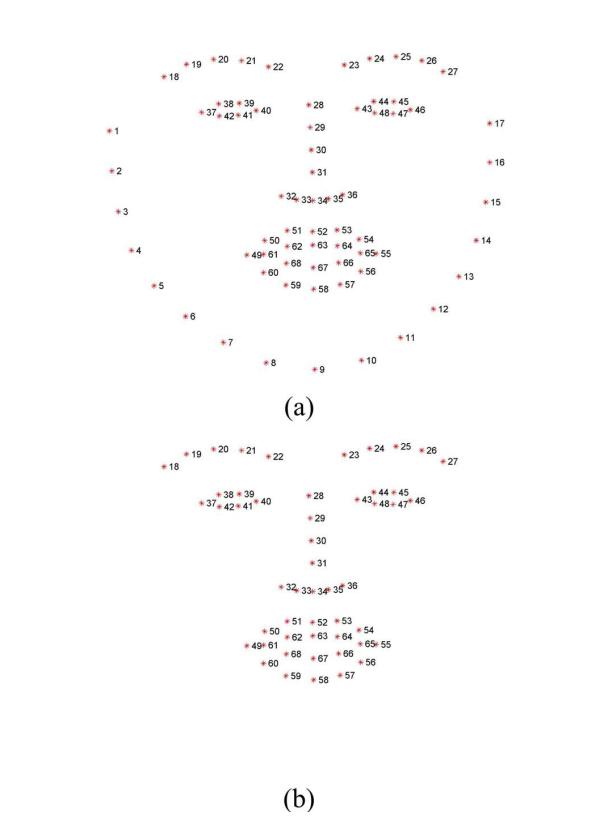
\includegraphics[width=0.5\textwidth]{img/33W.png}
        \caption{Conjunto de landmarks anotados en el dataset 300W, en la imagen \textit{a} contando el contorno del rostro son un total de 68 landmarks, en la imagen \textit{b} son 51 en total. Imagen extraida de \cite{300W}.}
        \label{fig:300W}
    \end{figure}
    
    \item \textbf{AFLW}: Se trata de un dataset de $24386$ imágenes \textit{in-the-wild} con un total de 21 landmarks anotados entre las cejas y el mentón, como podemos ver en la imagen \autoref{fig:AFLW}  \cite{AFLW}
    \begin{figure}[H]
        \centering
        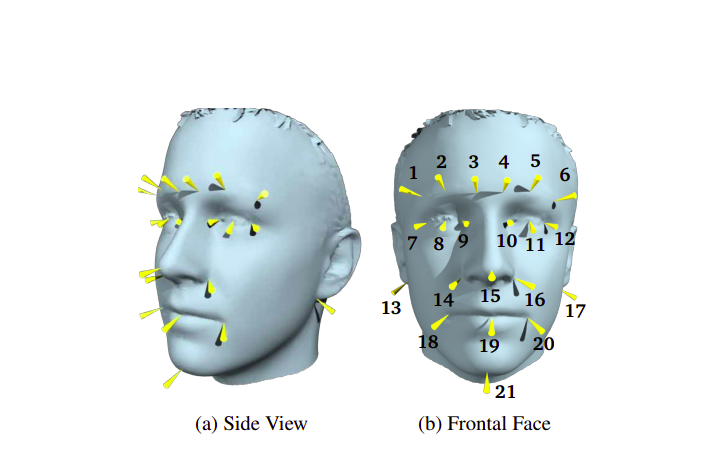
\includegraphics[width=0.8\textwidth]{img/AFLW.png}
        \caption{Conjunto de landmarks anotados sobre un modelo $3$D que emplea el dataset AFLW. Imagen extraida de \cite{AFLW}.}
        \label{fig:AFLW}
    \end{figure}
    \end{itemize}

    \medskip

    \noindent El hecho es que existen actualmente CNN que son capaces de reconocer con un alto grado de precisión estos conjuntos de landmarks marcados por las bases de datos anteriores, lo que nos hace pensar que quizá podría emplearse el conocimiento adquirido por estas redes para reentrenarlas en un proceso de \textit{fine-tuning} sobre una base de datos forense con landmarks anotados por un experto para tratar de resolver el problema de la identificación automática de landmarks. De ahí nace nuestra propuesta, que en cierto modo trata hace como nexo de unión entre las dos vías de investigación. 


\section{Framework empleado: 3FabRec }
        \noindent La red empleada para la resolución del problema es la desarrollada por \textbf{Bjorn Browatzki et al} en $2020$ \cite{browatzki20203fabrec} denominada \textbf{3FabRec}. La red en cuestión es un \textbf{Adversarial Autoencoder} combiando con una red \textit{GAN} (por la presencia de un segundo discriminante propio de las GANs) que puede predecir landmarks gracias a la incorporación de unas capas convolucionales intermedias denominadas \textit{Interleaved Transfer Layers} (ITLs) en la etapa de reconstrucción. Todos estos elementos serán explicados en profundidad más adelante.      

        \medskip

        \noindent Esta red aplica un método \textit{semi-supervisado} en el cual:

        \begin{itemize}
            \item Hay una primera fase de \textbf{aprendizaje no supervisado}, donde se pretende adquirir conocimiento implícito sobre la estructura facial contenida en grandes conjuntos de imágenes de rostros de personas en diversas posiciones, iluminación y etnia. Para ello se codifica todo este conocimiento implícito en un vector de un espacio latente de baja dimensionalidad para posteriormente reconstruir la imagen. Este proceso se hace íntegramente en el \textit{Adversarial Autoencoder}, sin hacer uso de las ITLs.
            \item Posteriormente, en una segunda fase de \textbf{aprendizaje supervisado}, se entrena la red con un conjunto de imágenes etiquetadas con landmarks faciales que la red tratará de predecir. Para ello se intercalan entre las capas del generador capas de convolución encargadas de reconstruir los mapas de calor de cada landmark junto con la reconstrucción del rostro del paso previo. Estas son las ITLs que mencionamos anteriormente.
            \item Finalmente, se puede incluir una tercera fase de \textit{finetuning} en la cual se entrena el Encoder para mejorar el rendimiento en la predicción de landmarks.
        \end{itemize} 

        \begin{figure}[H]
            \centering
            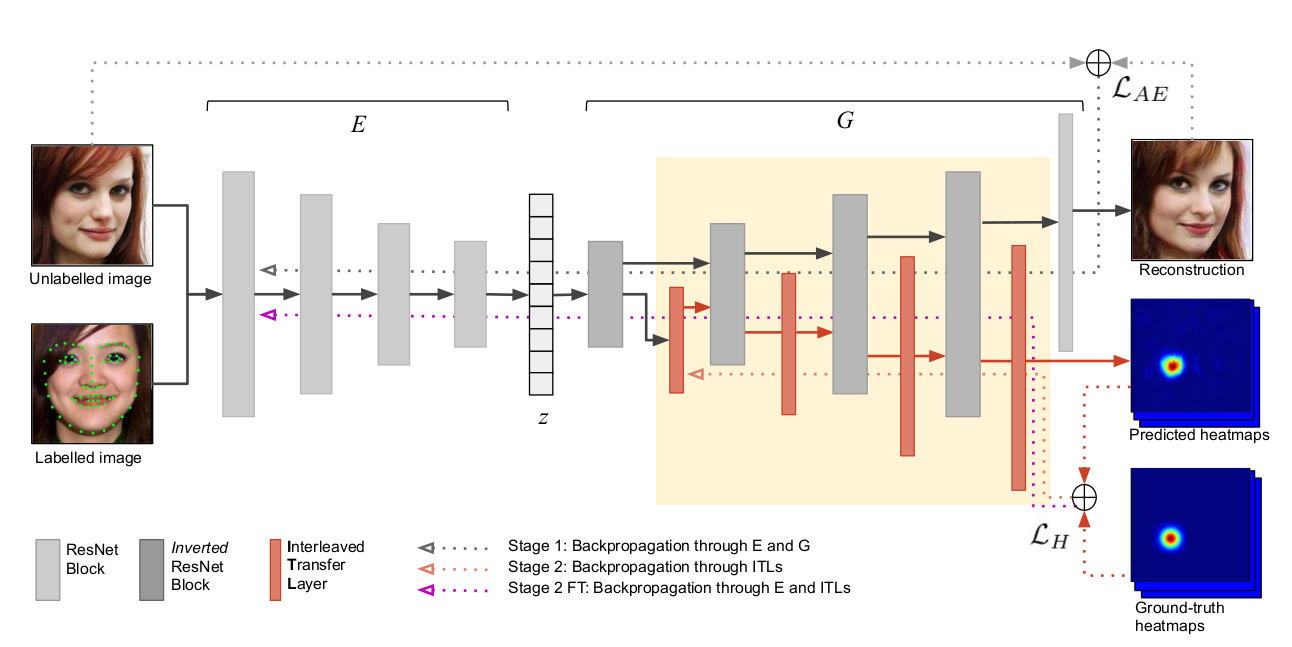
\includegraphics[width=0.98\textwidth]{img/3fabrec_arquitectura.png}
            \caption{Imagen resumen del framework 3FabRec. En ella podemos ver la estructura del \textit{Adversarial Autoencoder}, dividido en un Encoder (región bajo la \textit{E}) y un Generator (región bajo la \textit{G}). En rojo podemos ver las ITLs que se intercalan entre cada capa del Generador y dan como resultado un conjunto de mapas de calor. Imagen extraída de \cite{browatzki20203fabrec}.}
            \label{fig:3FabRec Resumen}
        \end{figure}

        \subsection{Arquitectura Adversarial Autoencoder}
            \noindent Para la construcción del \textit{Adversarial Autoencoder} utilizan:
            
            \begin{itemize}
                \item \textbf{Encoder}: emplean una ResNet-$18$  hasta codificar la entrada en un vector de $99$ dimensiones. Está pensado para imágenes de res $256 \times 256 \times 3$, aunque se adapta también a imágenes de dimensiones $512 \times 512 \times 3$.
                \item \textbf{Decoder}: emplean la misma red ResNet-$18$ pero invertida.
            \end{itemize}

            \noindent Para una mejor comprensión hemos realizado unos diagramas con la herramienta \textit{diagrams.net}. En la \autoref{fig:bloque_encoder} podemos ver la estructura básica de los bloques de la ResNet-$18$. Por otro lado en la \autoref{fig:Paso_encoder} podemos ver el paso de una imagen de entrada de tres canales y resolución $256 \times 256$ por el encoder.

            \begin{figure}[htbp]
                \centering
                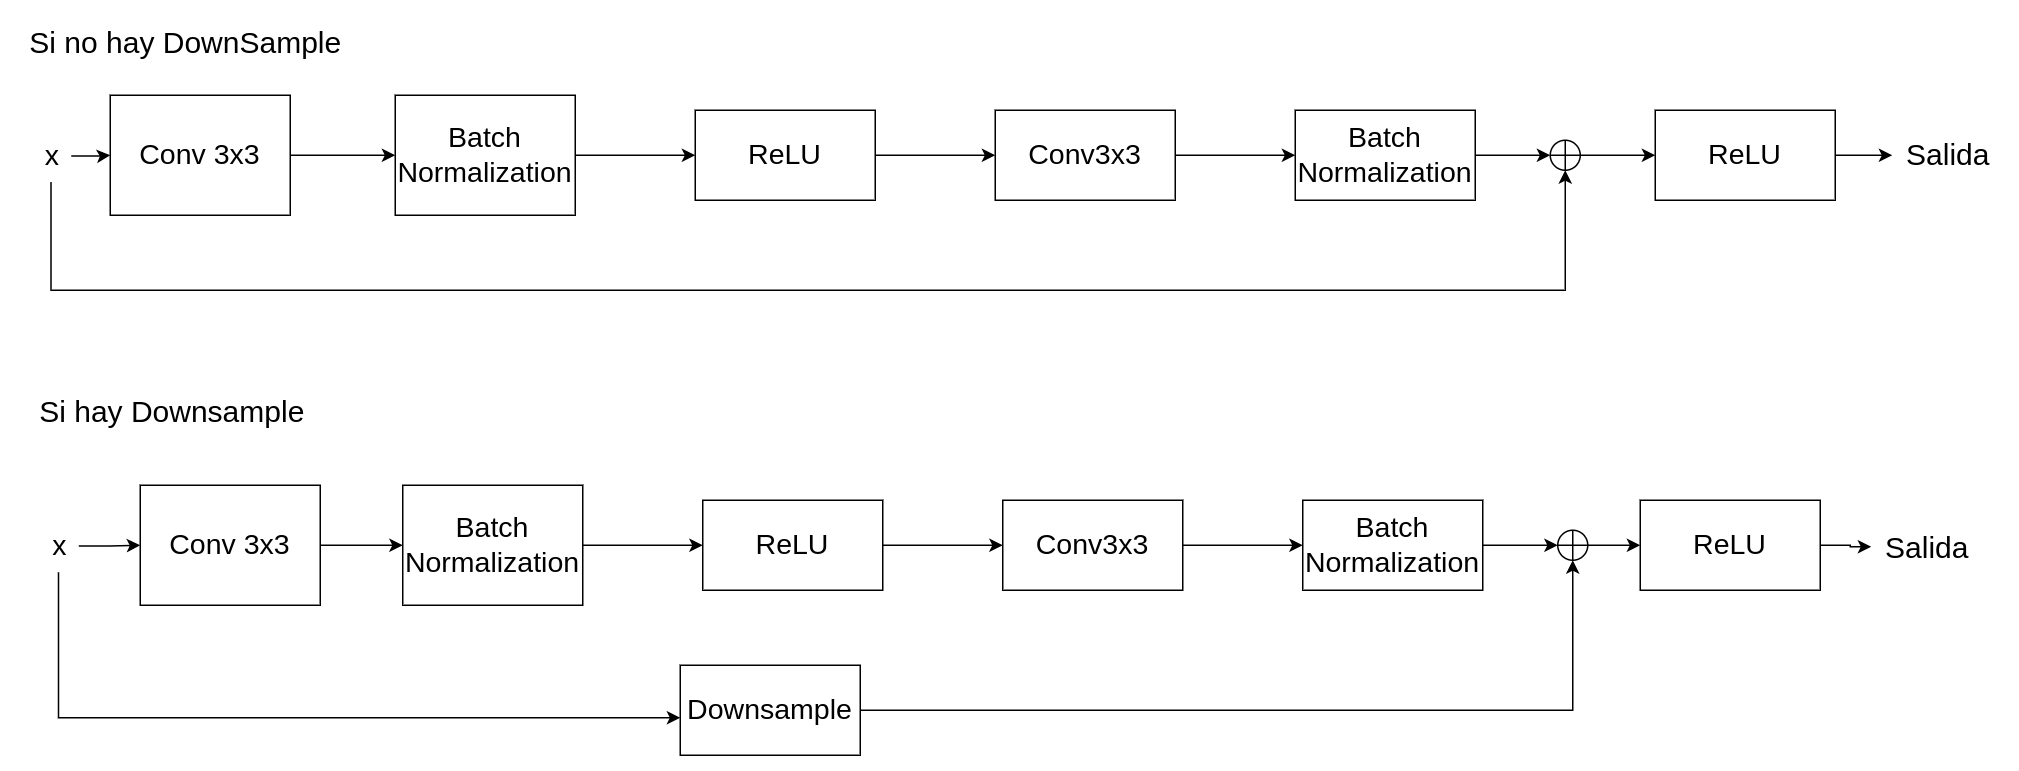
\includegraphics[width=0.95\textwidth]{img/bloque_basico_encoder.png}
                \caption{Bloques básicos que utilza la red ResNet-$18$ en sus capas. Se trata de una sucesión clásica de Convolución 3x3 + Batch Normalization + ReLU que se repite dos veces. En el primer caso los filtros de convolución no reducen las dimensiones del tensor añadiendo un padding de 1. En el segundo caso se reduce la dimensión del tensor a la mitad tras la primera convolución y se manteiene la dimensionalidad en la segunda. En el primer caso, la suma residual puede realizarse con el tensor x sin problema, en el segundo caso el tensor debe reducirse para que casen las dimensiones.}
                \label{fig:bloque_encoder}
            \end{figure}

            \begin{figure}[H]
                \centering
                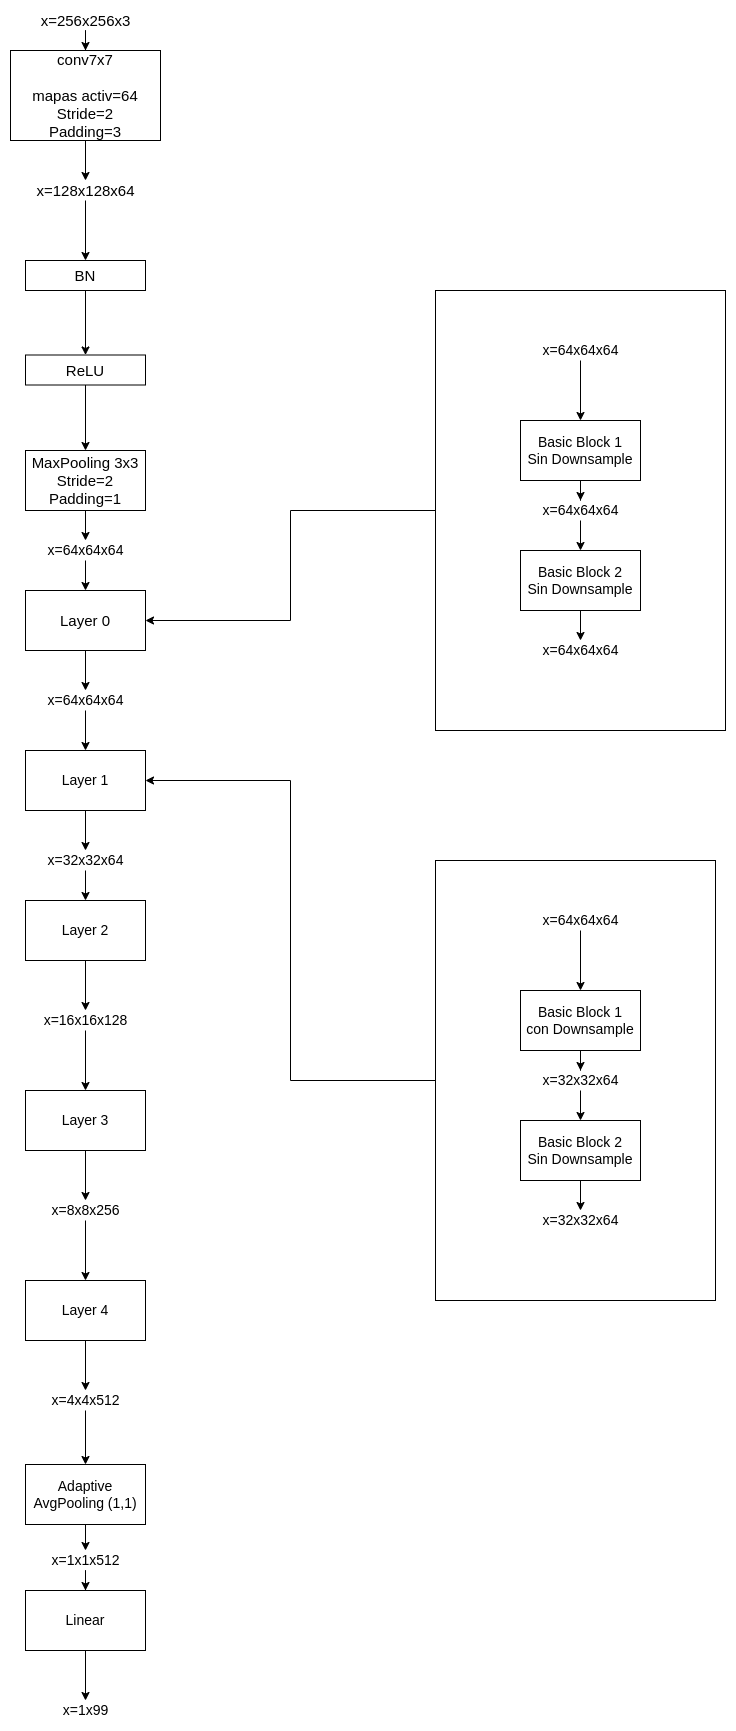
\includegraphics[width=0.7\textwidth]{img/3FabRec-Page-2.drawio.png}
                \caption{Ejemplo de paso de una imagen a través del Encoder. Cabe destacar que a partir de la Layer 1, todos los bloques tienen downsample.}
                \label{fig:Paso_encoder}
            \end{figure}

            \medskip

            \noindent En la \autoref{fig:Bloque_Decoder} podemos ver la estructura básica de un bloque en el Generador \textit{Inverse ResNet}, y un ejemplo del paso de un vector por el generador podemos verlo en la \autoref{fig:Paso_Generator}

            \begin{figure}[H]
                \centering
                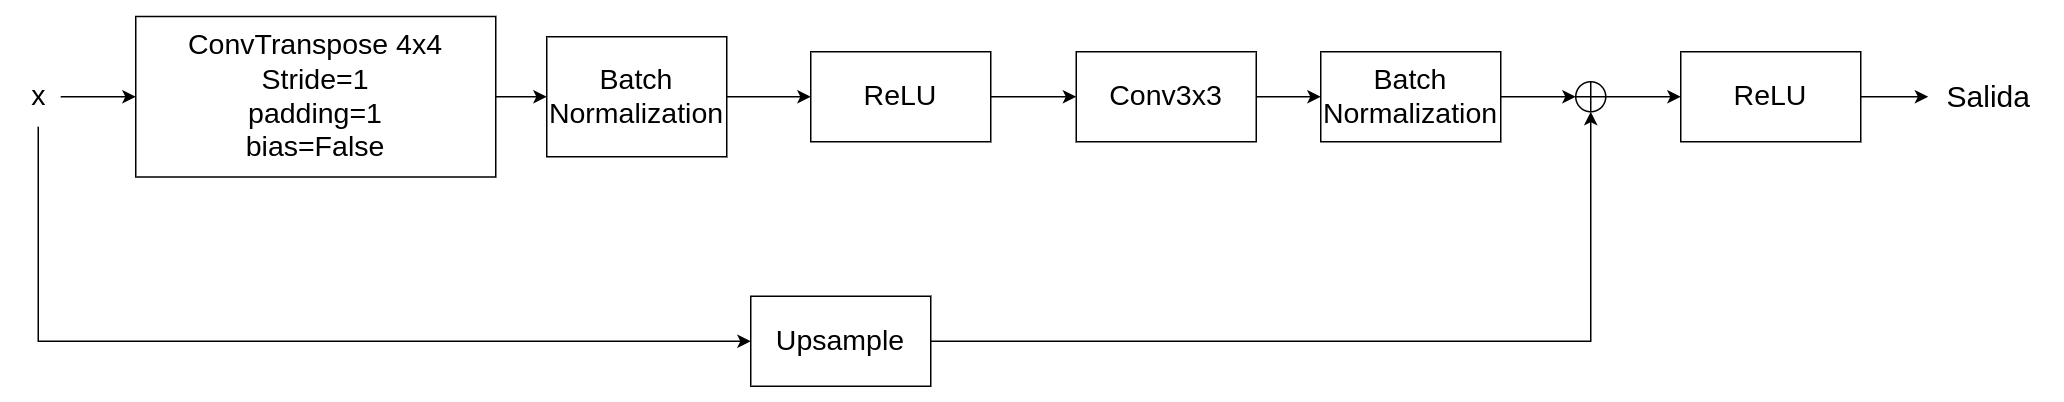
\includegraphics[width=0.96\textwidth]{img/bloque_invresnet.png}
                \caption{En primer lugar se aplica una convolución transpuesta que duplica las dimensiones del tensor de entrada y tras esto se sigue la misma estructura que en el bloque básico de la ResNet-$50$, la segunda convolución $3\times 3$ mantiene las dimensiones. Como consecuencia, para sumar el tensor de entrada con la salida del bloque se aumentan las dimensiones de este.}
                \label{fig:Bloque_Decoder}
            \end{figure}

            \begin{figure}[H]
                \centering
                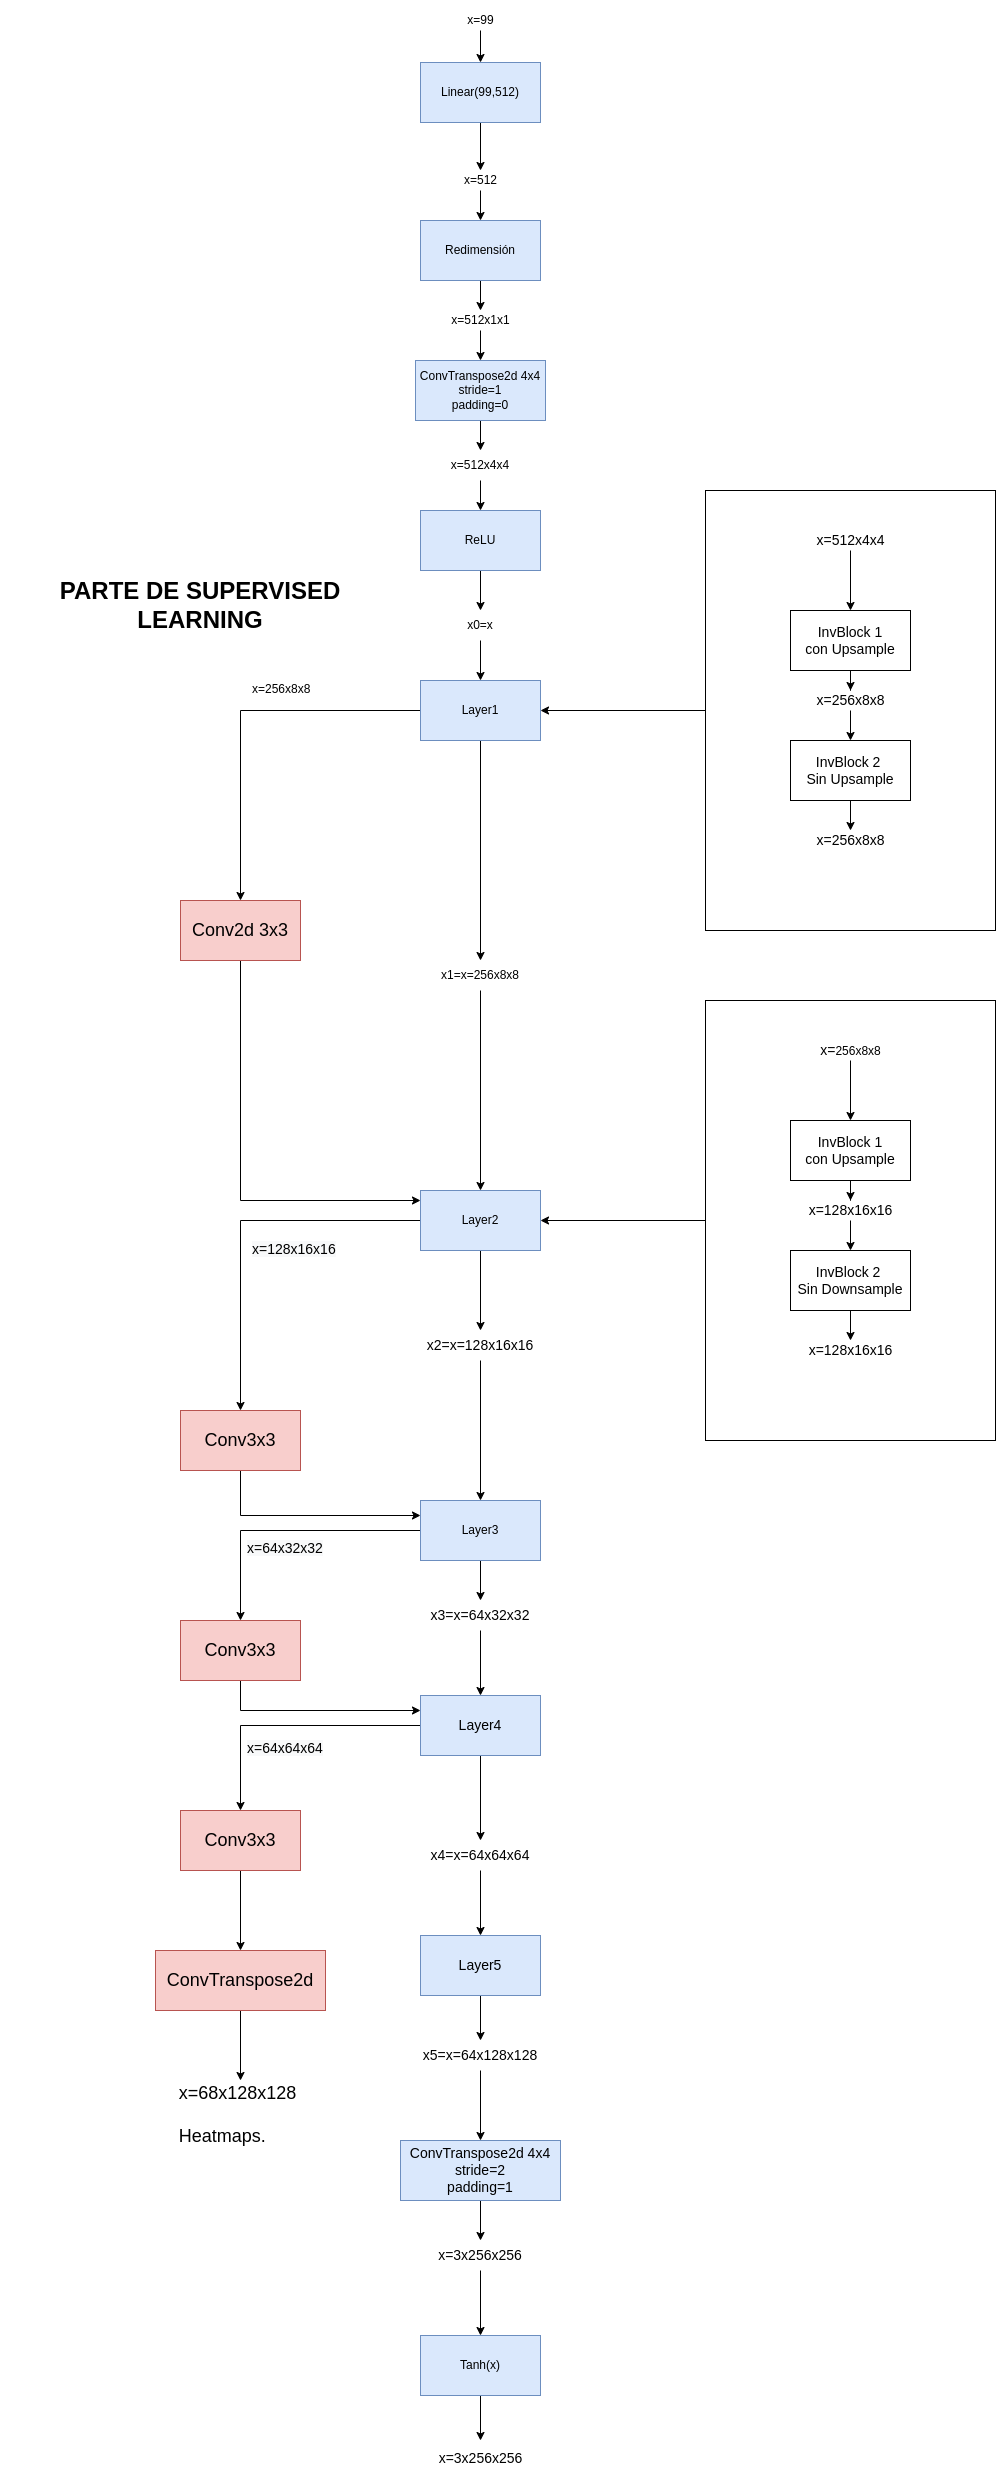
\includegraphics[width=0.95\textwidth]{img/paso_generator.png}
                \caption{Ejemplo del paso de un vector de $99$ dimensiones por el generador hasta reconstruirse la imagen de dimensiones $256 \times 256 \times 3$. La parte correspondiente al aprendizaje supervisado es la de los cuadrados azules, los cuadrados rojos corresponden a las \textit{ITLS} de la parte supervisada que se intercalan entre cada dos capas y dan como resultado los mapas de calor de los landmarks predichos.}
                \label{fig:Paso_Generator}
            \end{figure}

            \noindent Finalmente, para definir el autoencoder necesitamos un Discriminador, el cual que procure que los vectores del espacio vectorial latente sigan una determinada distribución. Dicha distribución será una normal multivariante estándar. Por otro lado, se añadirá un segundo discriminador propio de las redes \textbf{GAN} que nos dirá si la imagen reconstruida procede de la distribución que siguen los píxeles de la imagen de inicio. Este discriminador permite que la red genere imágenes más realistas, y es novedoso por no ser frecuente en la arquitectura de un Adversarial Autoencoder. En la \autoref{fig:DGaussian} las redes neuronales que definen ambos discriminadores.

            \begin{figure}[H]
                \centering
                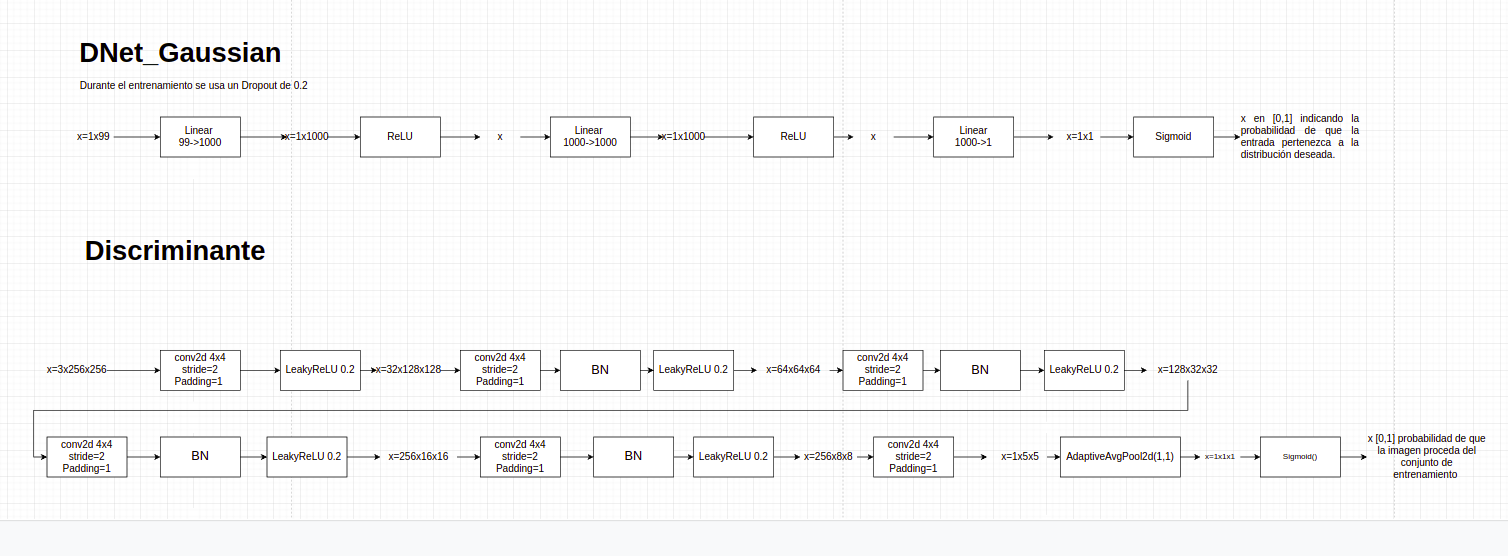
\includegraphics[width=0.95\textwidth]{img/DGaussian.png}
                \caption{En la imagen superior vemos el discriminante que se emplea para los vectores producidos por el Encoder y en la imagen inferior vemos el discriminante que se emplea para las imágenes generadas por el Generador. En ambos casos se da como salida un valor entre $0$ y $1$ que hace referencia a la probabilidad de pertenecer a la distribución deseada en el primer caso o a seguir la distribución de los píxeles de las imágenes en el segundo caso.}
                \label{fig:DGaussian}
            \end{figure}

            \subsubsection{Interleaved Transfer Layer (ITL)}
                \noindent Se denominan ITLs a las capas convolucionales encargadas de la predicción de landmarks. Se tratan de una solución novedosa porque premiten adaptar una AAE pensado originalmente para tareas de aprendizaje no supervisado a un problema de \textbf{regresión}, típico del aprendizaje supervisado.

                \medskip
                
                \noindent Se tratan de simples capas convolucionales que se intercalan entre las capas del Generador. La última de estas capas proporciona como salida un conjunto de mapas de calor, uno por cada landmark predicho. Estos mapas de calor luego se emplean para representar en la imagen reconstruida los landmarks. La arquitectura de esta etapa podemos verla en la \autoref{fig:Paso_Generator}.
            
        \subsection{Función de pérdida}

            \noindent La red utiliza dos funciones de pérdida, la primera que presentaremos se emplea en el entrenamiento del \textit{Adversarial Autoencoder}, en la parte no supervisada, y la segunda se utiliza tanto en la parte de aprendizaje supervisado como en la de \textit{fine-tuning} del Encoder. Debido al interés que tiene en el estudio del framework se van a presentar y explicar ambas funciones de pérdida. Cabe resaltar, que debido a que el problema que vamos a resolver es de \textbf{regresión}, en la fase de experimentación únicamente tendrá interés la segunda función de coste, asociada al entrenamiento de la parte supervisada.

            \medskip

            \noindent La función de pérdida empleada para el entrenamiento del \textit{Adversarial Autoencoder} en la parte de aprendizaje no supervisado es la siguiente: 
            
            \begin{align*}
                \min_{E,G} \max_{D_z,D_x} & \mathcal{L}_{AE}(E,G,D_z,D_x) = \\
                & \lambda_{rec} \mathcal{L}_{rec}(E,G) + \lambda_{cs}\mathcal{L}_{cs}(E,G) \\
                & + \lambda_{enc}\mathcal{L}_{enc}(E,D_z)+ \lambda_{adv} \mathcal{L}_{adv}(E,G,D_x)
            \end{align*}

            \noindent En la cual $\lambda_{enc}$ y $\lambda_{adv}$ toman el valor $1.0$ mientras que $\lambda_{rec}$ y $\lambda{cs}$ se establecen en $1.0$ y $60.0$ respectivamente. El valor de la función de coste se propagará por los pesos de $E$,$G$,$D_z$ y $D_x$ actualizándolos mediante \textit{back-propagation}. 

            \medskip

            \noindent Como podemos observar en la expresión anterior, se trata de una combinación lineal de cuatro funciones de coste distintas: 

            \begin{itemize}
                \item \textit{Error de reconstrucción}: Se trata de un error encargado de asegurarse de que la red reconstruya de forma apropiada las imágenes, para ello calcula la distancia $l_1$ entre la imagen original y la reconstruida pixel a pixel. Tiene la siguiente expresión, que coincide con la presentada en el apartado anterior de métricas.
                \begin{equation}
                    \mathcal{L}_{rec}(E,G)= \mathbb{E}_{x~p(x)}\left[\|x- G(E(x)) \|_1\right]
                \end{equation}
                \item \textit{Error estructural de la imagen}: Se trata de una variante del \textbf{SSIM} encargado de que la imagen real y la reconstruida tengan una estructura similar. Su expresión es la misma que la función presentada en la sección anterior de Métricas.
                \begin{equation}
                    \mathcal{L}_{cs}(E,G)= \mathbb{E}_{x~p(x)}\left[cs(x, G(E(x)))\right]
                \end{equation}
                \item \textit{Error del Encoder}: es el error empleado comunmente en este tipo de redes y que se asegura que el vector latente que genera el encoder siga la distribución impuesta en el discriminador $D_z$. Su expresión es:
                \begin{equation}
                    \mathcal{L}_{enc}(E,D_z)=\mathbb{E}_{z^*~p(z)}[\log(D_z(z^*))] + \mathbb{E}_{x~p(x)}[\log(1-D_z(E(x)))]
                \end{equation}
                \item \textit{Error adversario de imagen}: normalmente las imágenes generadas por los Autoencoders suelen generar imágenes emborronadas. Es por ello que se introduce este error, que añade un discriminador típico de una red \textit{GAN} que pretende discernir entre si la imagen que recibe como salida de la red pertenece al conjunto de imágenes de entrenamiento o si es una imagen generada por la red, de esta forma se generan imágenes más realistas. Su expresión es la siguiente: 
                \begin{equation}
                    \mathcal{L}_{adv}(E,D_z)=\mathbb{E}_{x~p(x)}[\log(D_x(x))] + \mathbb{E}_{x~p(x)}[\log(1-D_x(G(E(x))))]
                \end{equation}
            \end{itemize}

            \medskip

            \noindent Por otro lado, la función de pérdida que se empleará en el \textbf{entrenmiento de las \textit{ITLs}} será la siguiente: 

            \begin{equation} \label{eq::L2}
                \mathcal{L}_H(ITL) = \mathbb{E}_{x ~ p(x)} \left[ \| H-ITL(a)\|_2 \right]
            \end{equation}

            \noindent Dónde $a$ serían los mapas de activación que genera la ResNet invertida para la imagen codificada $z=E(x)$ (siendo $x$ la imagen de entrada a la red). En este caso se computa la distancia \textbf{$L_2$} entre los \textit{Heathmaps} de los lanmarks originales de la imagen $x$ de entrada, y los predichos por las \textit{ITLs}. Propagando el error por los pesos de las \textit{ITLS} solamente.

            \medskip

            \noindent A modo de aclaración, las imágenes etiquetadas con landmarks a la red suelen proporcionarse con el siguiente formato: 

            \begin{itemize}
                \item Un archivo con la imagen sin etiquetar. 
                \item Un archivo de texto plano con las coordenadas de cada landmark en la imagen.
            \end{itemize}

            \noindent Dados estos archivos, el framework, calcula para cada landmark proporcionado un mapa de calor en una imagen de tamaño $128 \times 128$ en el caso de que las imágenes de entrada sean de $256 \times 256$. Y es a ese conjunto de imágenes (una por cada landmark) a las que denominamos $H$ en la función anterior.

            \medskip

            \noindent Finalmente, en la etapa de \textit{fine-tuning} se computa la misma función de pérdida de antes, con la salvedad de que el error se propaga tanto por las \textit{ITLs} como por los pesos del \textit{Encoder}. Esto permite que el \textit{Encoder} se codifiquen con mayor precisión las imágenes y que se eliminen factores irrelevantes para la predicción de landmarks como son el género, el color de piel o la iluminación. Por otro lado se evita el overfitting ya que durante esta última etapa los pesos del \textit{Decoder} no se actualizan.

        \subsection{Proceso de entrenamiento de la red}

            \subsubsection{Entrenamiento no-supervisado}
                \noindent El framework que empleamos ha sido entrenado durante $50$ épocas con imágenes de tamaño $256x256$ y con un tamaño de batch de $50$. En todas las etapas del entrenamiento se ha empleado un optimizador tipo Adam, el cual durante el entrenamiento del \textit{Adversarial Autoencoder} usó $\beta_1=0.0$ y $\beta_2=0.999$ con un \textit{learning rate} de $2\times 10^{-5}$.

                \medskip

                \noindent Por otra parte, se aplicaron técnicas de \textit{data-augmentation} a las imágenes de entrada como giros horizontales, traslaciones, \textit{resizing} o rotaciones.

            \subsubsection{Entrenamiento supervisado}
                \noindent Para el entrenamiento de la parte supervisada, las imágenes de entrada se recortan de acuerdo a un \textit{bounding-box} creado por el framework a partir de unas coordenadas de entrada o bien de acuerdo a los landmarks que se proporcionan. Tras el recorte, se reescala la imagen hasta tener un tamaño de $256\times256$. 
                
                \medskip

                \noindent Por otro lado se crean los \textit{Heathmaps} para cada landmark. Para esto se crea una imagen de tamaño $128 \times 128$ por cada landmark marcando el punto con ayuda de una distribución normalde dos dimensiones centrada en las coordenadas del landmark y usando una desviación típica de $\sigma=7$.

                \medskip

                \noindent Tras esto se entrenan las cuatro \textit{ITLs}. A los datos de entrada se les aplican técnicas de \textit{data-augmentation} como rotaciones, traslaciones, reescalados y oclusiones. Para esta etapa se usa también un optimizador Adam con un \textit{learning rate} de $0.001$ y los mismos valores para $\beta_1$ y $\beta_2$.

                \medskip

                \noindent Finalmente, durante la etapa de \textit{fine-tuning} se establece un \textit{learning-rate} de $0.0001$ en las \textit{ITLs} mientras que el del \textit{Encoder} se mantiene en su valor por defecto de $2 \times 10^{-5}$ y cambiando el valor de $\beta_1 = 0.9$.

        \subsection{Bases de datos usadas por el framework}
            
            \noindent Para el entrenamiento no supervisado se emplearon los siguientes datasets unidos: 

            \begin{itemize}
                \item \textbf{VGGFace2} : Contiene un total de $3.3$ millones de imágenes de rostros en distintas poses, edad, iluminación, etnia, etc... Del dataset eliminaron las imágenes de rostros que tuviera una altura mayor a $100$ píxeles, quedando un total de $1.8$ millones de caras.
                \item \textbf{AffectNet} : Se trata de un dataset de $228$ mil imágenes en una gran variedad de poses, iluminación, etc..
            \end{itemize}

            \noindent En total usaron unas $2.1$ millones de imágenes.

            \noindent Para el entrenamiento supervisado se emplearon los siguientes datasets: 

            \begin{itemize}
                \item \textbf{300-W} : une diversos datasets de rostros etiquetados con \textbf{$68$}landmarks de manera semi-automática como son \textbf{LFPW},\textbf{AFW}, \textbf{HELEN} y \textbf{XM2VTS}. Además de añadir datos propios. En total emplearon $3,148$ (aproximadamente el $80 \%$ )imágenes para el entrenamiento y $689$ para test, las cuales se dividieron en dos grupos, uno de $554$ imágenes considerado el grupo test estándar, y otro de $135$ imágenes difíciles.
                \item \textbf{AFLW} : contiene un total de $24,386$ imágenes \textit{in-the-wild} con un amplio rango de poses distintas. Se emplearon $20,000$ (aproximadamente el $80 \%$) imágenes para test y $4,386$ para entrenamiento. Las imágenes vienen etiquetadas con $21$ landmarks, pero en el framework se entrena la red para predecir \textbf{$19$}.
                \item \textbf{WFLW}: Es la más reciente de las empleadas y tiene un total de $10,000$ imágenes. Se usan $7,500$ para entrenamiento y $2,500$ para test. Las imágenes tienen un total de \textbf{$98$} landmarks anotados.
            \end{itemize}

            \medskip

            \noindent Como podemos observar, los conjuntos de datos disponibles para el entrenamiento de redes especializadas en la identificación de landmarks faciales son variados y con muchos ejemplos de entrenamiento. En nuestro caso concreto, no contamos con tantos ejemplos y apenas hay bases de datos forenses con landmarks cefalométricos, lo cual es una dificultad añadida al problema, pues solo podremos entrenar con los datos que se nos proporcionan y como veremos son muy pocos.

\section{Métricas}

\noindent En esta sección, se van a presentar las principales métricas de error que se emplearán para estudiar la bondad de los resultados que se obtengan en futuros capítulos.

    \subsection{Métricas usadas en el entrenamiento}
        \noindent Las métricas que se muestran durante el entrenamiento utilizadas por el modelo son:

        \subsubsection{MSE}
            \noindent Se trata del error cuadrático medio, una función empleada típicamente en problemas de regresión y que tiene la siguiente expresión: 

            \begin{equation}
                MSE = \frac{1}{N} \sum_{i=1}^{N} (y_i - \widehat{y}_i)^2
            \end{equation}

            \noindent En nuestro caso concreto, este error se calcula entre los mapas de calor de los landmarks reales y predichos a nivel de pixel, es decir $y_i$ en la fórmula anterior corresponde a cada pixel del heatmap del landmark real y por tanto $\widehat{y}_i$ es el valor del pixel correspondiente en el heatmap predicho. Dichas diferencias se suman en todos los heatmaps y se divide por $N$ que en este caso es el número total de píxeles juntando todos los Heatmaps.

            \medskip

            \noindent Este error se empleará para realizar \textit{backpropagation} a través de las ITLs de la red y será el responsable del aprendizaje de la red.

    \subsection{Métricas empleadas en validación y testing}

        \subsubsection{Error de reconstrucción}
            \noindent Aunque no se trata de un métrica propia de un problema de regresión, el valor del error de reconstrucción en las imágenes de validación nos llevará en la sección de experimentación a realizar hipótesis sobre la relación entre este error y el NME.

            \medskip

            \noindent Se trata de la función de coste \textbf{L1} que se aplica a la imagen original y la reconstruida  y nos porporciona una medida del error de reconstrucción a nivel de pixel. Su expresión es la siguiente:

            \begin{equation}
                Reconstruction \; Loss = \sum_{i=1}^n |p_i -q_i|
            \end{equation}

            \noindent Dónde $p_i$ representa cada pixel de la imagen reconstruida por la red y $q_i$ el equivalente en la imagen real.

        \subsubsection{Normalized Mean Error}
            \noindent Este será el error utilizado para medir la bondad de los resultados. Tiene la siguiente expresión para cada landmark de los $30$: 

            \begin{equation}
                NME=\frac{\sqrt{\sum_{i=1}^{n}(p_{i,1} -q_{i,1})^2+ (p_{i,2} -q_{i,2})^2}}{N}
            \end{equation}


            \noindent Así, si en total se han identificado en las imágenes de validación un total de $n$ landmarks de cierto tipo en las imágenes de test o validación, se calcula la distancia $L_2$ entre el landmark de la imagen $i$ predicho y el real. Y tras esto se suman todos los valores obtenidos. Como podemos ver, idealmente $n$ debería ser el total de imágenes que hay en validación o test, pero no todos los landmarks aparecen en todas las imágenes, por lo tanto $n\leq M$ siendo $M$ el total de imágenes en validación.

            \noindent En dicha expresión $N$ es el término por el que se normaliza, y varía según el problema. En nnuestro caso normalizaremos la media del numerador por el ancho de la imagen que es de $256$ píxeles, ya que la distancia máxima permitida entre dos landmarks sería esta, y así todos los valores quedarían entre $0$ y $1$ siendo $0$ una estimación perfecta del landmark, y $1$ un error total en el marcado.

            \subsubsection{SSIM}
            \noindent Se trata del \textit{structural similarity index} (SSIM) y da una medida de \textit{similaridad} entre dos imágenes \cite{wang2004image}, su expresión es la siguiente: 

            \begin{equation}
                SSIM(x,y)=[l(x,y)]^\alpha[c(x,y)]^{\beta}[s(x,y)]^{\gamma}
            \end{equation}

            \medskip

            \noindent Dónde $x,y$ son las dos imágenes que van a ser comparadas.

            \medskip

            \noindent La componente $c(x,y)$ hace referencia a la función de comparación del contraste de las dos imágenes y viene dada por la siguiente expresión: 

            \begin{equation}
                c(x,y)=\frac{2\sigma_x \sigma_y + C}{\sigma_x^2+ \sigma_y^2+C}
            \end{equation}

            \noindent Dónde $\sigma_x, \sigma_y$ hacen referencia a la desviación estándar de cada imagen.

            \medskip

            \noindent La componente $s(x,y)$ es la función de comparación estructural entre las dos imágenes y viene dada por la siguiente expresión:

            \begin{equation}
                s(x,y)=\frac{\sigma_{xy}+C/2}{\sigma_x \sigma_y +C/2}
            \end{equation}

            \noindent Dónde $\sigma_{xy}$ denota la covarianza.

            \medskip

            \noindent La componente $l(x,y)$ hace referencia a la \textit{luminosidad}, pero en el caso de 3FabRec se prescinde de esta componente, además los exponentes $\alpha, \beta , \gamma$ se igualan a $1$.

            \medskip

            \noindent Por otra parte siguen las indicaciones del paper original de SSIM que recomiendan usar estas comparaciones en regiones de la imagen y promediarlas en vez de aplicarlas sobre todo el conjunto de píxeles de la imagen, es por ello que la expresión final queda:

            \begin{equation}
                cs(x,y)=\frac{1}{|w|} \sum{c(x_w,y_w)s(x_w,y_w)}_w
            \end{equation}

            \noindent Dónde $w$ representa la ventana sobre la que se aplica la función y $|w|$ el total de ventanas. En nuestro caso se emplean ventanas de tamaño $31\times 31$.

\section{Análisis de la base de Datos}
    \noindent En esta sección se van a presentar el dataset con los datos para resolver el problema principal de este trabajo, así como el análisis previo a la manipulación de los mismos y el preprocesamiento realizado.

    \subsection{Base de datos proporcionada}
        \noindent El conjunto de datos Forense que se proporciona para resolver el problema presenta las siguientes características: 

        \begin{itemize}
            \item Contienen un total de \textbf{167 imágenes} de distintos sujetos \textit{in-the-wild}. El número de imágenes por sujeto no se distribuye de forma equitativa, algunos solo disponen de una imagen mientras que otros tienen varias. El sujeto con mayor número de imágenes tiene siete.
            \item La resolución de las imágenes también varía mucho, oscilando entre los $4350 \times 3400$ píxeles y $168 \times 256$ píxeles.
            \item Hay imágenes a color y en escla de grises.
            \item Las imágenes se presentan en un conjunto muy variado de posiciones. Disponemos de: 
            \begin{itemize}
                \item $87$ imágenes frontales.
                \item $57$ imágenes con rostros en posición de \textbf{$3/4$}.
                \item $23$ imágenes de perfil.
            \end{itemize}
            \item Hay hasta un total de $30$ landmarks que pueden marcarse. Sin embargo, el número de landmarks en las imágenes es menor, como puede apreciarse en la \autoref{fig:Histograma}.
            \item En la \autoref{fig:Histograma} también podemos apreciar como la aparición de algunos landmarks es extremadamente baja, como es el caso del \textit{prosthion} y el \textit{Tragion} (tanto el izquierdo como el derecho). El resto de landmarks aparecen en más de la mitad de las imágenes. 
            \medskip
            \noindent La aparición en mayor o menor medida de cierto landmark en las imágenes nos sirve de indicador de si podrá ser o no aprendido por el modelo que usemos, de manera que los landmarks mencionados anteriormente, a causa del bajo número de ejemplos en los que aparecen puede ser más difícil que se aprendan.
        \end{itemize}
            \begin{figure}[H]
                \centering
                \includegraphics[width=0.5\textwidth]{img/imagenes_ejemplo_dataset.png}
                \caption{Imágenes de ejemplo del dataset proporcionado. Como puede observarse hay gran variedad de tamaños, poses, condiciones de iluminación diferentes que añaden dificultad al problema.}
                \label{fig:Imagenes_dataset}
            \end{figure}

            \begin{figure}[H]
                \centering
                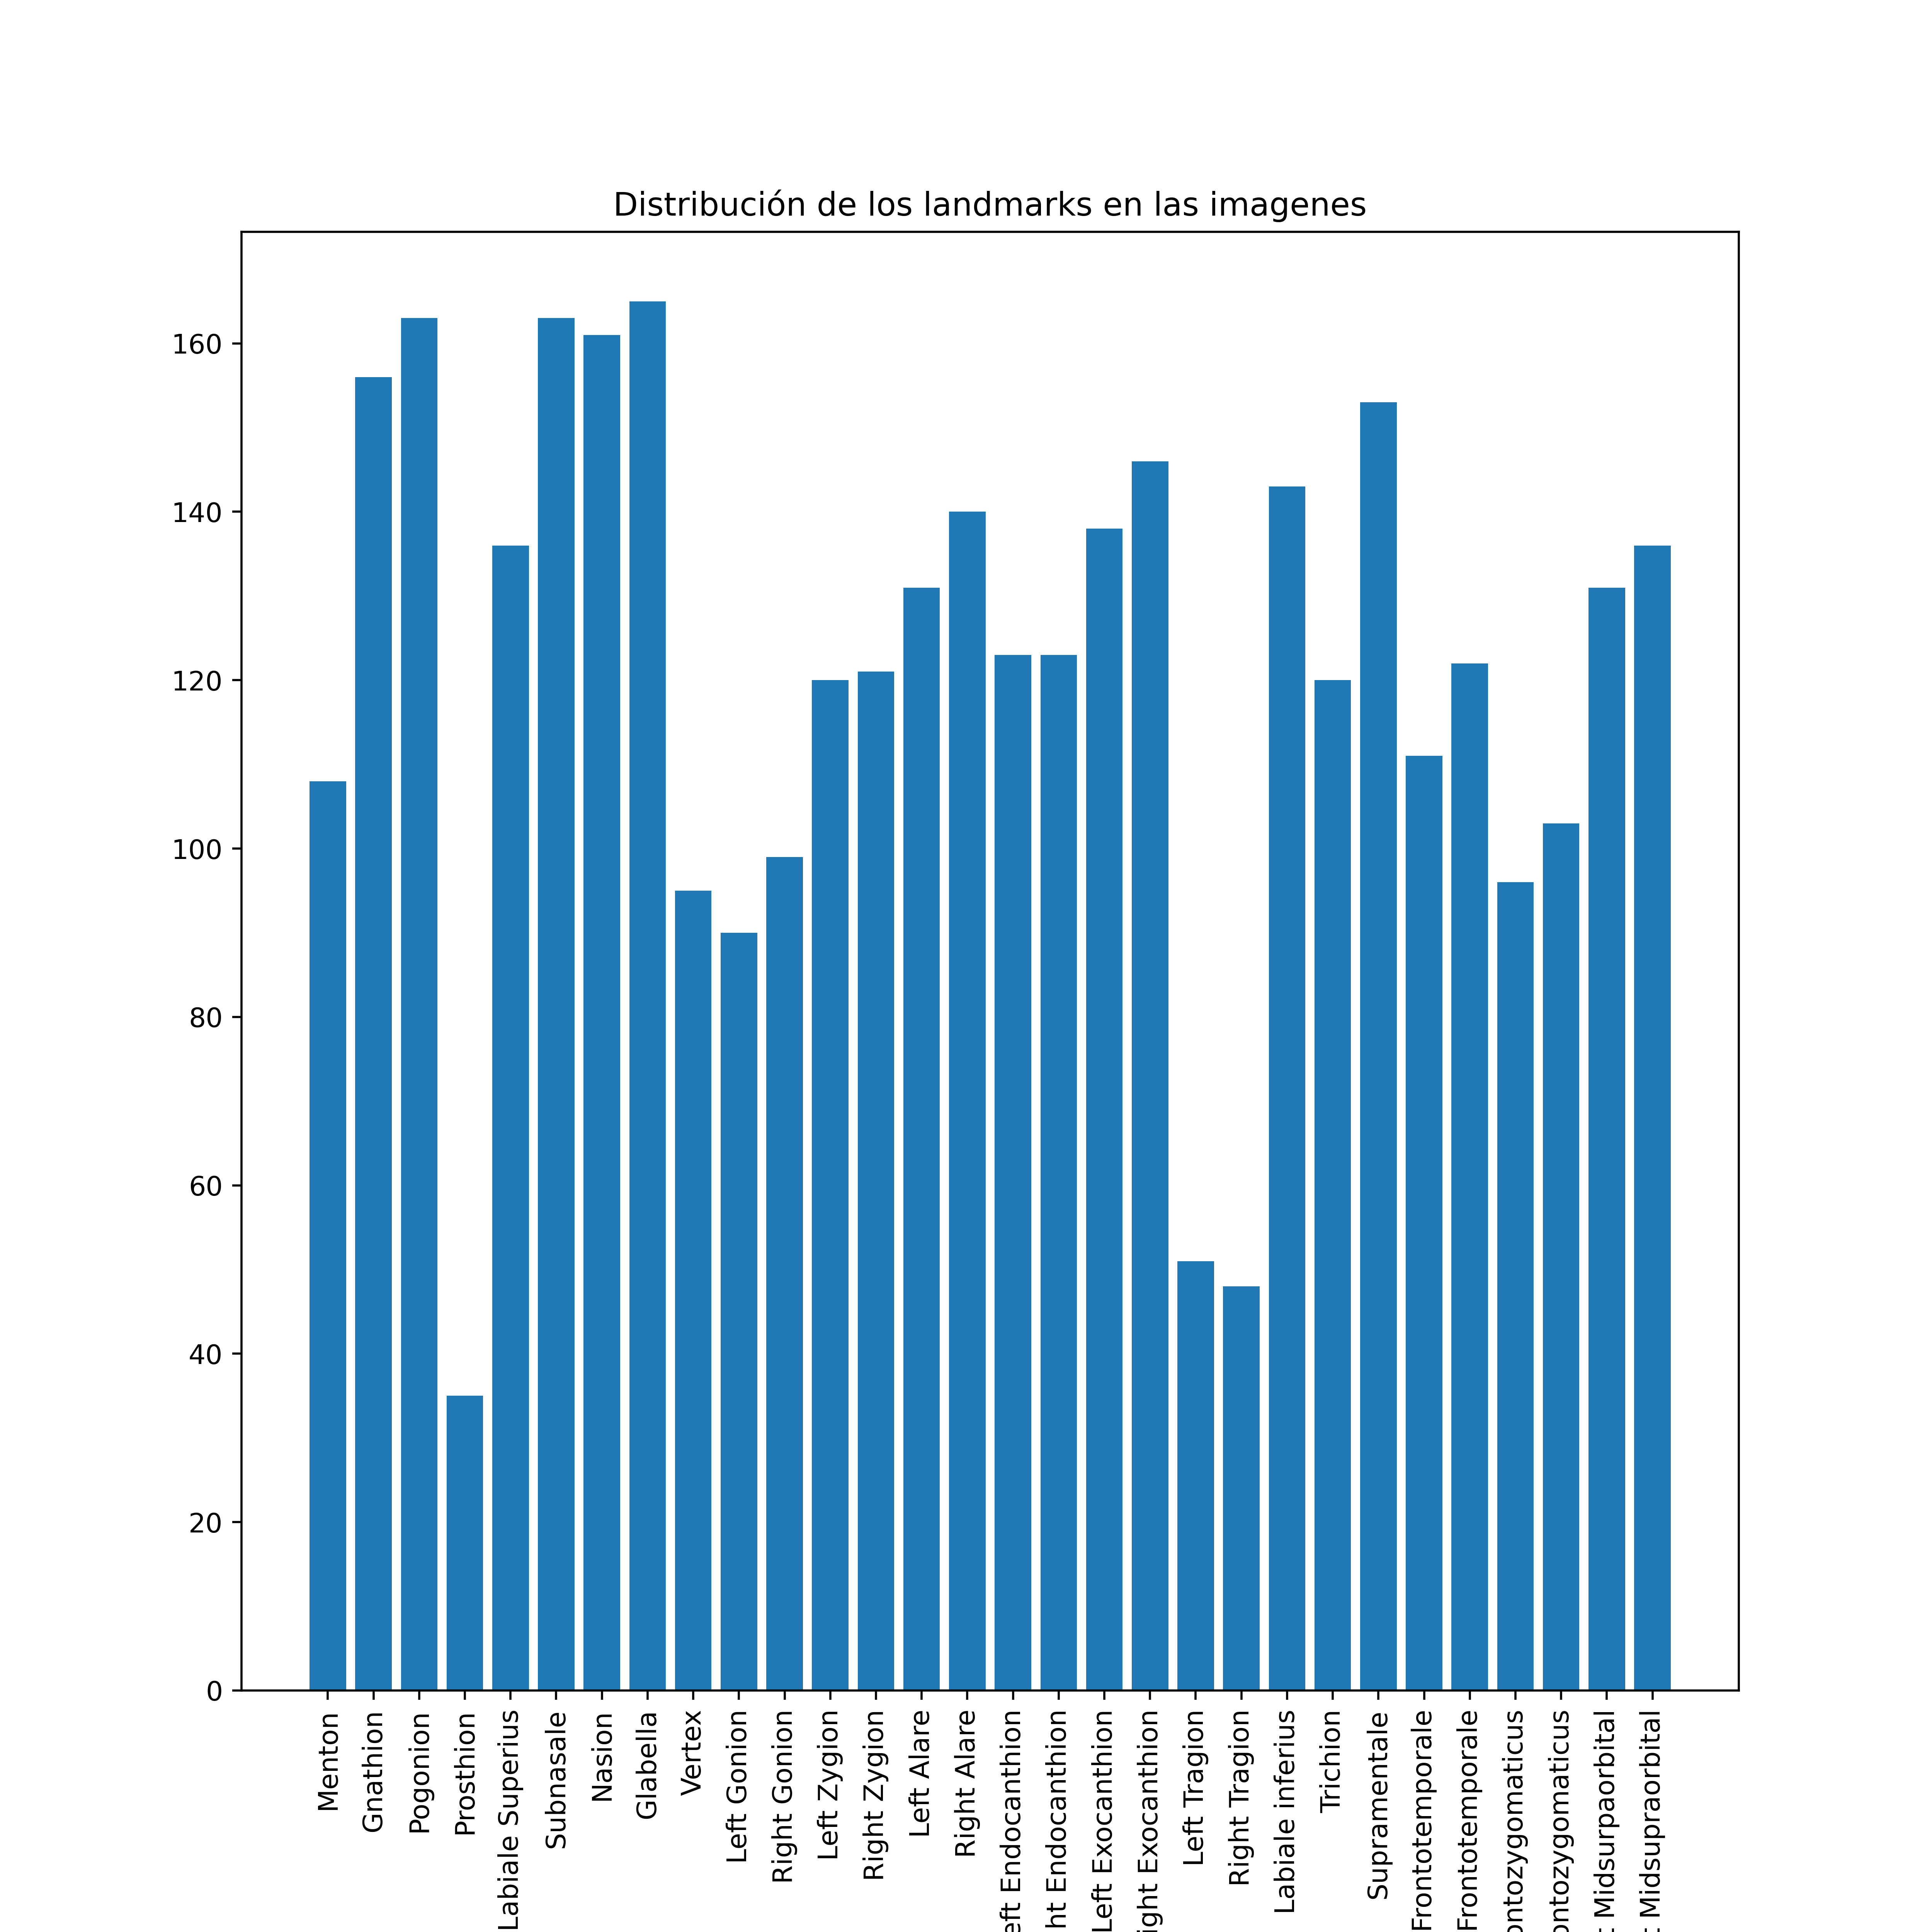
\includegraphics[width=0.7\textwidth]{img/distribucion_landmarks_imagenes.png}
                \caption{Histograma con la aparición de cada tipo de landmark en las imágenes del dataset.}
                \label{fig:Histograma}
            \end{figure}
    
    \subsection{Preprocesamiento}
        
        \subsubsection{Identificación de caras en las imágenes}
            \noindent Antes de poder entrenar el modelo, es necesario adecuar el dataset para que pueda usarse modelo. El framework está pensado para recibir como entrada una imagen, a la cual, se le hace un recorte a la región que ocupa el rostro con ayuda de un \textit{bounding box} predefinido y determinado por las coordenadas en la imagen de las cuatro esquinas o bien siguiendo los landmarks descritos por el fichero auxiliar asociado a cada imagen. En nuestro caso, debido a que la mayoría de landmarks son internos y no se suelen situar en los bordes de la cara, hemos pensado que la mejor manera de entrenar la red es que serealice el recorte de la imagen de entrada de acuerdo a un \textit{bounding box}. Para ello fue necesario emplear una red especializada en la detección de caras en imágenes y que nos proporcionaba como salida una lista con los \textit{bounding boxes} de todas las caras detectadas. La red se denomina \textbf{Facenet}, y se puede importar de la librería \textit{facenet} de \textit{pytorch} como \textit{mtcnn}.

            \medskip

            \noindent Así pues, se realizó un primer estudio para determinar los mejores parámetros para \textit{facenet}. Existen muchos parámetros editables, pero la mayoría se dejaron con sus valores por defecto, únicamente se consideró modificar: 

            \begin{enumerate}
                \item \textbf{image\_size}: Determina el tamaño de la imagen de salida.
                \item \textbf{select\_largest}: Si su valor es \textit{true}, se devuelve la cara más grande detectada, y si su valor es \textit{false}, se devuelve la de mayor confianza detectada.
            \end{enumerate}


            \noindent En nuestro caso, primero se probó con un \textit{image\_size} de $256 \times 256$, pero esto tenía problemas pues en ocasiones no podían construirse \textit{bounding boxes} de este tamaño y producían error, por lo que se redujo a $128 \times 128$. Por otro lado, observando las imágenes del dataset de entrenamiento, nos dimos cuenta que en algunas imágenes aparecían varios sujetos, y en ocasiones la cara más \entrecomillado{grande} mo pertenecía al sujeto principal. Es por ello que se decidió establecer el parámetro \textit{select\_largest} a \textit{False}, y así obtener como salida una lista de \textit{bounding boxes} ordenados de mayor a menor según el nivel de confianza. No obstante, en algunos casos se tuvo que elegir con cuidado cuál de los bounding boxes proporcionados se correspondía con el sujeto principal.

            \medskip

            \noindent Una vez establecidos los parámetros, se detectaron problemas en la identificación de caras en algunas imágenes. Debido a que todas las imágenes erróneas estaban en escalas de grises nos dimos cuenta de que la red sólo acepta como entrada imágenes en tres canales, por lo que cada imagen en escala de grises de un solo canal tuvimos que replicar tres veces su canal. 
        
            \medskip
        
            \noindent Tras esto, volvimos a ver que en algunas imágenes no se detectaban \textit{bounding boxes}. Esto nos llevó a realizar un breve estudio sobre si era buena idea continuar usando esta red o buscar otra. En este estudio clasificamos las imágenes en tres grupos y aplicamos la red a cada uno de ellos por separado: 

            \begin{enumerate}
                \item Imágenes de sujetos en posición \textbf{ frontal}: en total hay $87$ imágenes frontales de las cuales se extraen correctamente el \textbf{$100\%$} de los \textit{bounding boxes}.
                \item Imágenes de sujetos en posición de \textbf{$3/4$}: En este caso hay $57$ imágenes de las cuales el \textbf{$100\%$} de los \textit{bounding boxes} extraidos por la red son correctos.
                \item Imágenes de sujetos en posición de \textbf{perfil}: En este caso hay un total de $23$ imágenes y se clasifican correctamente $20$, lo que supone una precisión del \textbf{$87\%$}. Además, las imágenes que fallaban estaban en escala de grises y con malas condiciones de calidad e iluminación.
            \end{enumerate}

            \noindent Por lo tanto, debido al bajo número de ejemplos en los que la red falla, se decidió mantener la red \textbf{Facenet} para determinar los \textit{bounding boxes} y además se excluyeron los tres ejemplos dónde fallaba del dataset, lo que hizo que en total se usaran $164$ de las $167$ imágenes originales.

            \medskip 

            \begin{figure}[H]
                \centering
                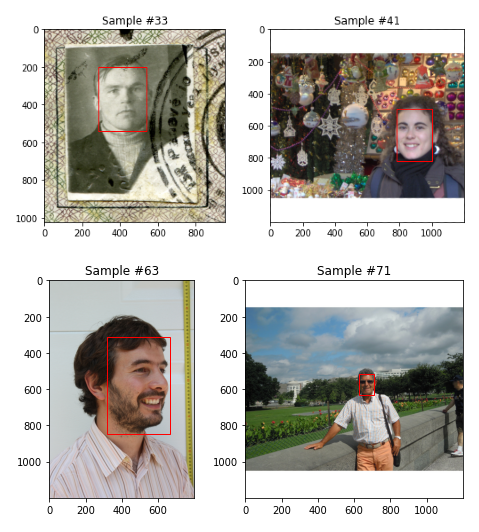
\includegraphics[width=0.7\textwidth]{img/imagenes_ejemplo_bb.png}
                \caption{Imágenes de ejemplo del dataset con los \textit{bounding boxes} marcados por \textit{Facenet}. Como podemos observar, aunque son correctos, los \textit{bounding boxes} marcados recortan excesivamente los límites del rostro, pudiendo incluso eliminar partes en las que hay landmarks marcados. Las imágenes han sido generadas con \textit{matplotlib}.}
                \label{fig:Ejemplo_bb}
            \end{figure}

            \noindent Durante el estudio anterior, se observaron otros hechos dignos de mención. En primer lugar se identificaron dos imágenes repetidas, pero se decidió mantenerlas pues los landmarks presentes en una y otra eran diferentes, lo que podía ayudar al entrenamiento. Por otro lado, durante el entrenamiento se vió cómo había una imagen de un determinado sujeto en la que aprecían simultáneamente dos fotos, una  de frente y otra de perfil. Sin embargo, al estar los landmarks anotados únicamente en la imagen de frente se tomó el \textit{bounding box} de la imagen frontal desechando el otro para el perfil. En otras dos imágenes se pueden ver un conjunto de varias personas, y la red mostraba erróneamente los \textit{bounding boxes} de personas que no eran el sujeto de estudio, por lo que estudiar cuál de todos los \textit{bounding boxes} devueltos pertenecía al sujeto correcto.

        \subsubsection{Creación del fichero annotations en el dataset}

            \noindent Una vez se identificaban correctamente todos los \textit{bounding boxes}, siguiendo como inspiración el dataset \textit{AFLW}, se generó un fichero denominado \textit{annotations.csv} dentro de la carpeta del proyecto en el que encuentra el dataset. En este fichero se almacenó \textbf{para cada imagen} una serie de datos: 

            \begin{itemize}
                \item El nombre del fichero.
                \item El índice de la imagen dentro del dataset. 
                \item Una lista con las coordenadas $2D$ de cada landmark en la imagen (incluidos los no presentes como situados en la posición $[-1,-1]$). 
                \item Una lista denominada máscara, que representa la visibilidad de cada landmark en la imagen. Los landmarks visibles en la imagen tienen asociado el valor $1$, mientras que los no visibles tienen asociado el valor $0$. Esta máscara será de gra utilidad a la hora de extraer las métricas, pues hay que realizar las medias de acuerdo al número de landmarks visibles de cada tipo, no se puede usar siempre el valor $30$.
                \item Finalmente, se almacena la posición de las cuatro esquinas que definen el \textit{bounding box}, para que el framework recorte la imagen quedándose con el rostro únicamente. 
            \end{itemize}

        \subsubsection{Reajuste de los bounding boxes}
            \noindent Finalmente, como parte del proceso de determinar los \textit{bounding boxes}, se vió que en todos los casos, dichos rectángulos cortaban parte de las caras de los sujetos. En ocasiones partes en las que había landmarks marcados, es por ello, que se tuvo que realizar una transformación del \textit{bounding box} sugerido para que manteniendo el centro del mismo abarcase una mayor superficie y que contuviera el rostro completo del sujeto. 

            \medskip

            \noindent La transfomación consiste en desplazar la esquina superior izquierda del rectángulo una cantidad \textit{m} en el eje de ordenadas y abscisas y establecer el resto de esquinas de acuerdo a este parámetro como se muestra en la \autoref{fig:Transformacion_BB}.


            \begin{figure}[H]
                \centering
                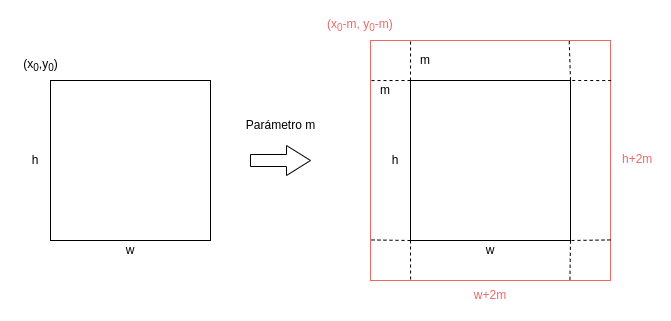
\includegraphics[width=0.8\textwidth]{img/Transformacion_rectangulo.png}
                \caption{Proceso seguido para la transformación.}
                \label{fig:Transformacion_BB}
            \end{figure}

            \begin{figure}[H]
                \centering
                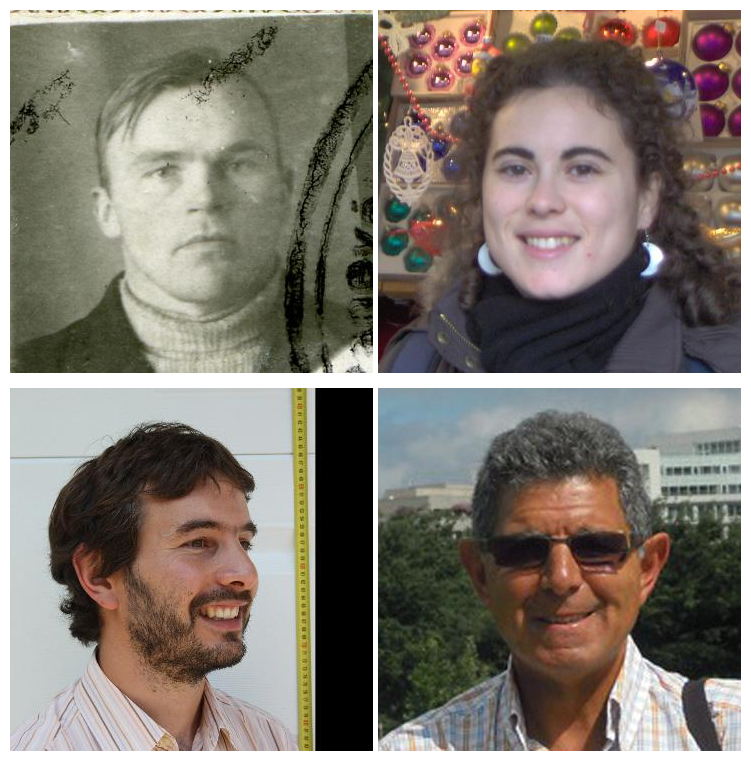
\includegraphics[width=0.7\textwidth]{img/imagenes_ejemplo_cropping.png}
                \caption{Recorte de las caras tras el reajuste del \textit{bounding box}.}
                \label{fig:Reajuste_bb}
            \end{figure}



    \subsection{Separación en conjuntos de entrenamiento y validación}
        \noindent En primer lugar ,separaremos el conjunto de datos que se proporciona en conjuntos de entrenamiento, validación y test. Debido a que trabajaremos con un conjunto de datos reducido será necesario emplear \textbf{validación cruzada} para la elección entre los modelos que se prueben. Así pues, de las \textbf{164 imágenes} que usaremos en total, establecemos una semilla para que los procesos aleatorios sean replicables en cualquier máquina y con ayuda de la función \textit{random-shuffle} de python separamos los datos en: 

        \begin{itemize}
            \item \textbf{Conjunto de test}: 33 imágenes ($20\%$ del total de imágenes).
            \item \textbf{Conjunto de entrenamiento:} 131 imágenes ($80\%$ del total de imágenes).
        \end{itemize}

        \noindent Por otro lado, el conjunto de entrenamiento se subdivide a su vez en cinco subconjuntos, con la idea de realizar \textbf{5-fold cross-validation}. Cada subconjunto estará compuesto por \textbf{26 imágenes} exceptuando el último que tendrá \textbf{27}.
        
        \medskip

        \noindent Para esta técnica se realizan cinco ejecuciones independientes en la cual se toman cuatro de los cinco subconjuntos de entrenamiento para entrenar el modelo y se deja el último subconjunto para validar el modelo. Con esta técnica, en cada iteración se cambia el conjunto que se empleará para validación, con la finalidad de mejorar la calidad de las decisiones que se tomen sobre el rendimiento, pues la decisión estará mejor informada. 

        \medskip

        \noindent De esta manera, con cada propuesta de modelo que realicemos, se medirá su rendimiento usando \textbf{5-fold cross-validation}, obteniendo 5 salidas de validación para cada modelo. La elección del mejor será mediante el cómputo de la mediana de estos para cada mdelo.


\section{Experimentación}
    \subsection{Hipótesis iniciales}
        \noindent Debido a que partimos de \textbf{3fabRec}, un framework diseñado y probado de forma exahustiva por Björn Browatzki y Christian Wallraven, en los experimentos se va a respetar la arquitectura de la red en su totalidad, sin añadir ni eliminar capas. Del mismo modo, debido a que la elección del optimizador \textbf{Adam} empleado por los autores ha sido fruto de un proceso de experimentación exahustiva por parte de los mismos no, se va a probar a cambiarlo. Además, el optimizador Adam es adaptativo y tiene muy buen rendimiento en general, por lo que no tenemos ninguna razón que nos lleve a pensar que lograríamos grandes mejoras cambiando de optimizador.

        \medskip

        \noindent También, en la creación de los \textit{Heat maps} se ha optado por mantener el valor de $\sigma =7$ que se recomienda en el paper \cite{browatzki20203fabrec}, ya que de nuevo ha sido probado minuciosamente por los autores del framework.
    
    \subsection{Modelo Base}
        \noindent Buscamos un \textbf{modelo base} con el que obtener los primeros resultados, y que iremos refinando hasta obtener el modelo solución. El framework \textbf{3FabRec} viene por defecto con cuatro modelos. Todos ellos han sido entrenados en la fase de aprendizaje no supervisado. Uno de ellos viene sin entrenamiento posterior de landmarks en ningún dataset, y los otros tres vienen con un entrenamiento en los datasets \textit{300w}, \textit{AFLW} y \textit{WFLW}. Así pues, la primera decisión a tomar es si emplear un modelo preentrenado en alguno de los datasets o utilizar uno sin entrenar. 

        \medskip

        \noindent Los tres datasets anteriores han sido ya estudiados en apartados anteriores, y finalmente se ha optado por usar como modelo base el que ha sido entrenado en \textit{AFLW}. Esto se debe a que el número de landmarks que predice este modelo es similar al de nuestro problema, ya que predice 21 landmarks. Por otro lado, los landmarks de AFLW, pese a no tener una justificación biológica, son parecidos a los anotados en el dataset que se proporciona. Es por esto que consideramos una buena primera decisión emplear la red \textbf{preentrenada en AFLW}.

        \medskip

        \noindent Por otro lado, debido a que no conocemos todavía el efecto que tiene el entrenamiento con la etapa de \textit{ajuste fino} del encoder sobre los datos, vamos a realizar un entrenamiento únicamente de las \textbf{ITLs} durante un total de \textbf{40 épocas}, valor a partir del cual se aprecia la convergencia del \textit{mse} (que recordamos, es la medida de error entre los \textit{Heat maps} predichos por el modelo y los reales), y no utilizaremos técnicas de \textit{data augmentation}. Por otro lado, los parámetros que se han usado han sido los que sugieren por defecto en el framework, ya que aún no tenemos información suficiente sobre el rendimiento como para cambiarlos. Dichos valores son: 

        \begin{itemize}
            \item El \textit{learning rate} para el optimizador Adam usado en el entrenamiento de las ITLs se establece en $0.001$. 
            \item El valor del parámetro $\beta_1$ se establece en $0.0$.
            \item El valor del parámetro $\beta_2$ se establece en $0.9$.
        \end{itemize}

        \noindent Los resultados obtenidos por imagen en cada partición de \textbf{cross validation 5-fold } se pueden encontrar en \autoref{ap:apendiceA}. En estas tablas podemos observar la media del NME obtenido entre todos los landmarks presentes en la imagen, los no marcados no computan. Los resultados obtenidos son en general buenos para ser el modelo base. El NME no es muy elevado, aunque el error de reconstrucción y estructural sí lo son. Podemos concluir así que no se están reconstruyendo fielmente las imágenes a nivel de píxel, aunque como vemos en la \autoref{fig:Ejemplo_ModelBase}, la reconstrucción de las caras es apropiada en general. No obstante, esto podría afectar al marcado de landmarks, puesto que estos se marcan en primer lugar sobre la imagen reconstruida, y luego se trasladan a la original.

        \begin{table}[!ht]
            \centering
            \caption{Media del error NME obtenido por landmark entre todas las particiones de cross-validation.}
            \begin{tabular}{|l|l|l|}
            \hline
                ~ & \cellcolor{gray!25}\textbf{Landmark} & \cellcolor{gray!25}\textbf{Media NME por landmark} \\ \hline
                0 & Menton & 3.944 \\ \hline
                1 & Gnathion & 2.637 \\ \hline
                2 & Pogonion & 2.549 \\ \hline
                3 & Prosthion & 0.932 \\ \hline
                4 & Labiale Superius & 2.099 \\ \hline
                5 & Subnasale & 2.059 \\ \hline
                6 & Nasion & 2.254 \\ \hline
                7 & Glabella & 2.547 \\ \hline
                8 & Vertex & 6.244 \\ \hline
                9 & Left Gonion & 7.684 \\ \hline
                10 & Right Gonion & 11.283 \\ \hline
                11 & Left Zygion & 5.098 \\ \hline
                12 & Right Zygion & 6.309 \\ \hline
                13 & Left Alare & 1.939 \\ \hline
                14 & Right Alare & 2.282 \\ \hline
                15 & Left Endocanthion & 1.668 \\ \hline
                16 & Right Endocanthion & 1.671 \\ \hline
                17 & Left Exocanthion & 1.706 \\ \hline
                18 & Right Exocanthion & 1.670 \\ \hline
                19 & Left Tragion & 4.824 \\ \hline
                20 & Right Tragion & 5.376 \\ \hline
                21 & Labiale inferius & 1.705 \\ \hline
                22 & Trichion & 4.478 \\ \hline
                23 & Supramentale & 1.913 \\ \hline
                24 & Left Frontotemporale & 2.319 \\ \hline
                25 & Right Frontotemporale & 2.721 \\ \hline
                26 & Left Frontozygomaticus & 1.513 \\ \hline
                27 & Right Frontozygomaticus & 2.313 \\ \hline
                28 & Left Midsurpaorbital & 1.205 \\ \hline
                29 & Right Midsupraorbital & 1.43 \\ \hline
            \end{tabular}
            \label{table:ModelBase_landmarkresume}
        \end{table}

        \medskip

        \noindent Los resultados por landmark se puden ver en la \autoref{table:ModelBase_landmarkresume} y son buenos en general para tratarse del modelo base, siendo el landmark mejor marcado en media el \textit{Prosthion}, y el peor el \textit{Right Gonion}. Si recordamos la \autoref{fig:Histograma}, sorprende el hecho de que el \textit{Prosthion} es de los landmarks que menos presencia tiene en las imágenes (aparece en menos de $40$ imágenes), y sin embargo es de los que mejor aprende a marcar la red. Por otro lado, el \textit{Right Gonion}, pese a aparecer en unas $100$ imágenes, resulta más dificil para la red predecirlo. Esto puede deberse a que las imágenes con mayor error de reconstrucción son las de perfil, y es en este tipo de imágenes en las que mejor se aprecia dicho landmark.

        \medskip

        \noindent Por otro lado, podemos ver en la \autoref{fig:Curvas_modelbase} las curvas de aprendizaje de cada partición. Todas tiene una gran capacidad de generalización, pues como vemos el error de validación desciende a la par que el de entrenamiento y está poco por encima de este último.

        \begin{figure}[H]
            \centering
            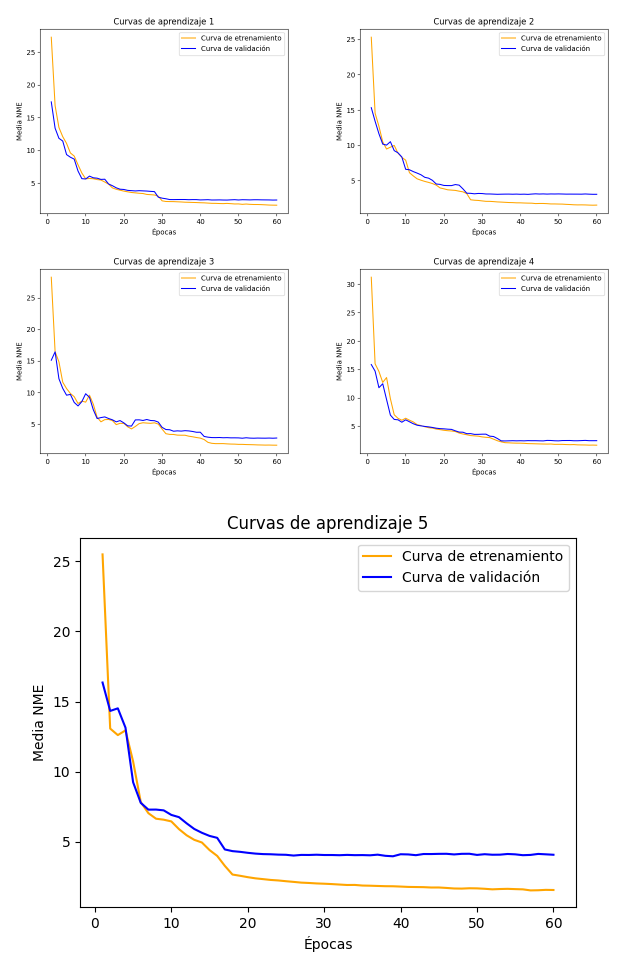
\includegraphics[width=0.9\textwidth]{img/curvas_aprendizaje_modelbase.png}
            \caption{Curvas de aprendizaje en cada partición del modelo base.}
            \label{fig:Curvas_modelbase}
        \end{figure}

        \noindent En resumen, los resultados parecen buenos para tratarse de una primera aproximación. Sin embargo, consideramos que debido a la gran variabilidad del dataset tanto en posturas, como en calidad e iluminación de imagen, la reconstrucción de las imágenes se ha resentido, especialmente en las imágenes de perfil. Esto provoca que el modelo también marque peor los landmarks, por lo que vamos a intentar mejorar esto en los próximos modelos. Podemos ver el rendimiento del modelo en algunas imágenes en la \autoref{fig:Ejemplo_ModelBase}.

        \begin{figure}[H]
            \centering
            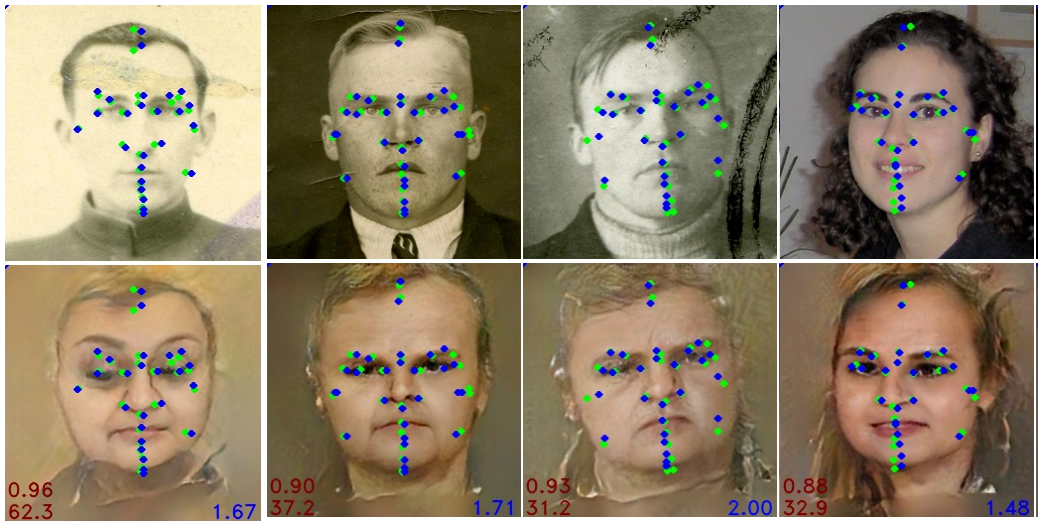
\includegraphics[width=0.9\textwidth]{img/image_basemodel.png}
            \caption{Imágenes pertenecientes a distintos conjuntos de validación para el \textbf{modelo base}. Las imágenes de la fila superior son las imágenes reales, y las de la fila inferior las reconstruidas por la red. El marcado se realiza sobre las reconstruidas y luego se lleva a las superiores. Podemos apreciar en verde los landmarks reales y  en azul los predichos. El valor que aparece en la esquina inferior derecha es el NME global de la imagen (la media de los NMEs de cada landmark) y en la esquina inferior izquierda aparece el error de reconstrucción y encima el SSIM.}
            \label{fig:Ejemplo_ModelBase}
        \end{figure}

    \subsection{Modelo con reentrenamiento del encoder}
        \noindent A la luz de los resultados anteriores, vamos a cambiar el modelo de manera que ahora junto con las ITLs (que seguirán usando el mismo optimizador con los mismos parámetros por defecto), vamos a entrenar los pesos del \textit{encoder}. Con este enfoque queremos enseñar a la red a \textbf{codificar mejor} la información presente en las imágenes del dataset (que, son más difíciles que las de los datasets empleados anteriormente), a la par que la enseñamos a marcar landmarks en las mismas. Remarcamos, que la función de coste que se empleará tanto para el entrenamiento de los pesos de las ITLs como los del encoder será el \textit{MSE} entre los mapas de calor predichos y los reales.

        \medskip

        \noindent Es importante aclarar que este proceso no produce overfitting, pues durante las etapas de entrenamiento los pesos del \textit{decoder} permanecerán congelados, y serán únicamente los pesos del \textit{encoder} los que se actualicen con backpropagation. El optimizador empleado para el entrenamiento del \textit{encoder} es Adam, el mismo que ellos emplean y los parámetros se mantienen por defecto ($\beta_1=0.9$ y $\beta_2=0.999$) a excepción del \textit{learning rate}, que se establece a $2^{-6}$, en vez de $2^{-5}$. El motivo por el cual se realiza este cambio es porque experimentando en esta fase se vio que con el antiguo \textit{Learning rate} no se conseguía mejorar apenas la reconstrucción en validación, pues durante el entrenamiento el error de reconstrucción pronto quedaba estancado en un valor. Para evitar esto se optó por reducir el learning rate consiguiendo mejorar un poco más el error de reconstrucción. El entrenamiento duró en total \textbf{100 épocas}, pues como veremos, el modelos mejora más lentamente en el reconocimiento de landmarks.

            \begin{table}[!ht]
                \centering
                \caption{Tabla comparativa entre los dos modelos explorados por ahora. Medimos el NME medio a nivel de landmark. En verde se resalta el mejor valor de marcado para cada landmark, en un verde más intenso las mejoras más considerables.}
                \begin{tabular}{|l|l|l|l|}
                \hline
                    \textbf{} & \cellcolor{gray!25}\textbf{Landmark} & \cellcolor{gray!25}\textbf{Media NME (Modelo base)} & \cellcolor{gray!25}\textbf{Media NME (Modelo Encoder)} \\ \hline
                    \textbf{0} & Menton & \cellcolor{green!25} 3.944 & 3.997 \\ \hline
                    \textbf{1} & Gnathion & 2.637 & \cellcolor{green!25} 2.606 \\ \hline
                    \textbf{2} & Pogonion & 2.549 & \cellcolor{green!25} 2.546 \\ \hline
                    \textbf{3} & Prosthion & \cellcolor{green!25} 0.932 & 1.048 \\ \hline
                    \textbf{4} & Labiale Superius & 2.099 & \cellcolor{green!25} 2.04 \\ \hline
                    \textbf{5} & Subnasale & 2.059 & \cellcolor{green!25} 1.992 \\ \hline
                    \textbf{6} & Nasion & 2.254 & \cellcolor{green!25} 2.099 \\ \hline
                    \textbf{7} & Glabella & \cellcolor{green!25} 2.547 & 2.736 \\ \hline
                    \textbf{8} & Vertex & 6.244 &\cellcolor{green!25} 5.89 \\ \hline
                    \textbf{9} & Left Gonion & 7.684 & \cellcolor{green!50} \textbf{5.789} \\ \hline
                    \textbf{10} & Right Gonion & 11.283 & \cellcolor{green!50} \textbf{5.301} \\ \hline
                    \textbf{11} & Left Zygion & \cellcolor{green!25} 5.098 & 5.288 \\ \hline
                    \textbf{12} & Right Zygion & 6.309 & \cellcolor{green!25} 6.291 \\ \hline
                    \textbf{13} & Left Alare & \cellcolor{green!25} 1.939 & 1.959 \\ \hline
                    \textbf{14} & Right Alare & 2.282 & \cellcolor{green!25} 2.232 \\ \hline
                    \textbf{15} & Left Endocanthion & \cellcolor{green!25} 1.668 & 1.71 \\ \hline
                    \textbf{16} & Right Endocanthion & 1.671 & \cellcolor{green!25} 1.647 \\ \hline
                    \textbf{17} & Left Exocanthion & \cellcolor{green!25} 1.706 & 1.733 \\ \hline
                    \textbf{18} & Right Exocanthion & \cellcolor{green!25} 1.670 & 1.746 \\ \hline
                    \textbf{19} & Left Tragion & 4.824 & \cellcolor{green!25} 3.633 \\ \hline
                    \textbf{20} & Right Tragion & 5.376 & \cellcolor{green!25} 5.252 \\ \hline
                    \textbf{21} & Labiale inferius & 1.705 & \cellcolor{green!25} 1.688 \\ \hline
                    \textbf{22} & Trichion & \cellcolor{green!25} 4.478 & 4.762 \\ \hline
                    \textbf{23} & Supramentale & \cellcolor{green!25} 1.913 & 1.991 \\ \hline
                    \textbf{24} & Left Frontotemporale & \cellcolor{green!25} 2.319 & 2.452 \\ \hline
                    \textbf{25} & Right Frontotemporale & \cellcolor{green!25} 2.721 & 3.282 \\ \hline
                    \textbf{26} & Left Frontozygomaticus & 1.513 & \cellcolor{green!25} 1.499 \\ \hline
                    \textbf{27} & Right Frontozygomaticus & \cellcolor{green!25} 2.313 & 2.516 \\ \hline
                    \textbf{28} & Left Midsurpaorbital & 1.205 & \cellcolor{green!25} 1.178 \\ \hline
                    \textbf{29} & Right Midsupraorbital & 1.43 & \cellcolor{green!25} 1.348 \\ \hline
                \end{tabular}
                \label{table:Encode_landmarkresume}
            \end{table}    

    \noindent Como podemos observar en la \autoref{table:Encode_landmarkresume}, los valores son muy similares a los del modelo base, pese a que este ha entrenado durante más épocas. El \textit{Prosthion} sigue siendo el landmark mejor marcado, con un valor del error NME ligeramente superior al del modelo base. Sin embargo la verdadera mejora se aprecia en el marcado de landmarks de los perfiles, al mejorar la reconstrucción de los mismos, el \textit{Right Gonion} ha bajado su error a la mitad, y el \textit{Left Gonion} ha reducido su error en dos puntos con respecto al modelo base.
    
    \medskip
    
    \noindent Por otro lado, como podemos ver en las tablas de validación por imágenes en el \autoref{ap:apendiceB}, el error de reconstrucción ha mejorado muy ligeramente en las imágenes de validación, y no supone una mejora considerable con respecto al modelo base, ocurriendo lo mismo con el error estructural.

    \medskip

    \noindent Finalmente podemos observar las curvas de aprendizaje para este modelo en la \autoref{fig:curvas_encoder}. A diferencia del modelo anterior, comienza a bajar la capacidad de generalización a partir de la época 20 aproximadamente. El error de entrenamiento comienza a descender muy lentamente con cada época mientras que el de validación se mantiene constante.

    \begin{figure}[H]
        \centering
        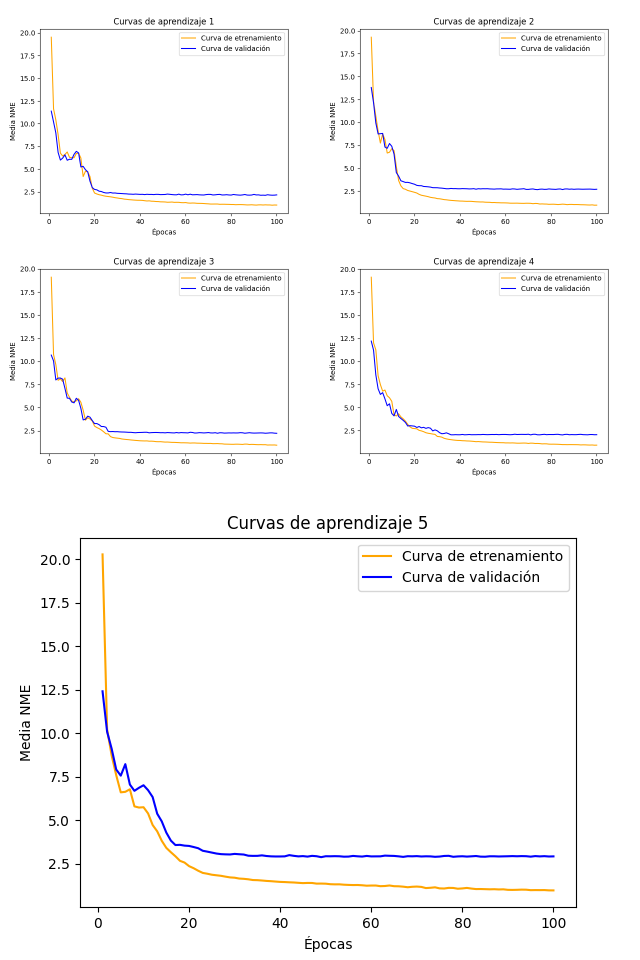
\includegraphics[width=0.9\textwidth]{img/curvas_encoder.png}
        \caption{Curvas de aprendizaje en cada partición del modelo de finetuning del encoder.}
        \label{fig:curvas_encoder}
    \end{figure}

    \medskip

    \noindent Viendo estos resultados no parece muy prometedora esta línea de investigación. Bien es cierto que hemos mejorado considerablemente el error de los dos landmarks peor marcados, pero el coste computacional que ha supuesto no compensa para la leve mejora global del modelo. Es por esto por lo que vamos a cambiar el enfoque sobre el \textit{fine-tuning} en el siguiente modelo. Podemos ver el comportamiento del modelo en algunas imágenes de validación de diversas particiones de \textit{cross-validation} en la \autoref{fig:Ejemplo_encoder}

    \begin{figure}[H]
        \centering
        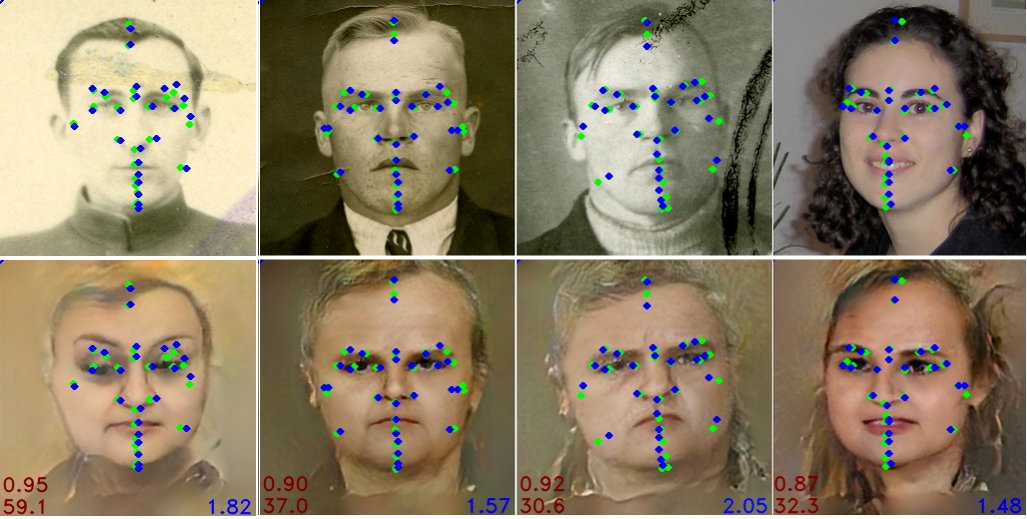
\includegraphics[width=0.9\textwidth]{img/image_encoder.png}
        \caption{Imágenes pertenecientes a distintos conjuntos de validación para el \textbf{modelo de ajuste fino del encoder}.}
        \label{fig:Ejemplo_encoder}
    \end{figure}

    \subsection{Modelo con reentrenamiento del decoder}
        \noindent Del mismo modo en que se experimentó con el \textit{encoder} se hizo con el \textit{decoder}. En este enfoque asumimos que el framework sabe codificar correctamente las imágenes pero que no realiza lo suficientemente bien la reconstrucción de las mismas debido a la alta variabilidad del dataset. Esta etapa es completamente análoga a la del modelo anterior (incluyendo el mismo tipo de optimizadores, parámetros y regiones que permanecen congeladas de la red), pero actualizando los pesos del \textit{decoder} y las ITLs mientras se congelan los pesos del \textit{encoder}.

        \begin{table}[!ht]
            \centering
            \caption{Tabla comparativa entre los tres modelos probados. En este caso no se aprecia ninguna mejora considerable con respecto a las introducidas por el modelo de ajuste fino del encoder}
            \begin{tabular}{|l|l|l|l|l|}
            \hline
                \textbf{} & \cellcolor{gray!25}\textbf{Landmark} & \cellcolor{gray!25}\textbf{M.Base} & \cellcolor{gray!25}\textbf{M.Encoder} & \cellcolor{gray!25}\textbf{M.Decoder} \\ \hline
                \textbf{0} & Menton & 3.944 & 3.997 & \cellcolor{green!25} 3.991 \\ \hline
                \textbf{1} & Gnathion & 2.637 & \cellcolor{green!25} 2.606 & 2.634 \\ \hline
                \textbf{2} & Pogonion & 2.549 & \cellcolor{green!25} 2.546 & 2.585 \\ \hline
                \textbf{3} & Prosthion & \cellcolor{green!25} 0.932 & 1.048 & 0.97 \\ \hline
                \textbf{4} & Labiale Superius & 2.099 & \cellcolor{green!25} 2.04 & 2.059 \\ \hline
                \textbf{5} & Subnasale & 2.059 & \cellcolor{green!25} 1.992 & 2.089 \\ \hline
                \textbf{6} & Nasion & 2.254 & \cellcolor{green!25} 2.099 & 2.275 \\ \hline
                \textbf{7} & Glabella & \cellcolor{green!25} 2.547 & 2.736 & 2.912 \\ \hline
                \textbf{8} & Vertex & 6.244 & \cellcolor{green!25} 5.89 & 6.137 \\ \hline
                \textbf{9} & Left Gonion & 7.684 & 5.789 & \cellcolor{green!25} 5.665 \\ \hline
                \textbf{10} & Right Gonion & 11.283 & \cellcolor{green!25} 5.301 & 5.468 \\ \hline
                \textbf{11} & Left Zygion & \cellcolor{green!25} 5.098 & 5.288 & 5.29 \\ \hline
                \textbf{12} & Right Zygion & 6.309 & 6.291 & \cellcolor{green!25} 6.14 \\ \hline
                \textbf{13} & Left Alare & \cellcolor{green!25} 1.939 & 1.959 & 2.051 \\ \hline
                \textbf{14} & Right Alare & 2.282 & \cellcolor{green!25} 2.232 & 2.295 \\ \hline
                \textbf{15} & Left Endocanthion & \cellcolor{green!25} 1.668 & 1.71 & 1.827 \\ \hline
                \textbf{16} & Right Endocanthion & 1.671 & 1.647 & \cellcolor{green!25} 1.61 \\ \hline
                \textbf{17} & Left Exocanthion & \cellcolor{green!25} 1.706 & 1.733 & 1.809 \\ \hline
                \textbf{18} & Right Exocanthion & \cellcolor{green!25} 1.670 & 1.746 & 1.734 \\ \hline
                \textbf{19} & Left Tragion & 4.824 & \cellcolor{green!25} 3.633 & 4.163 \\ \hline
                \textbf{20} & Right Tragion & 5.376 & 5.252 & \cellcolor{green!25} 4.791 \\ \hline
                \textbf{21} & Labiale inferius & 1.705 & 1.688 & \cellcolor{green!25} 1.627 \\ \hline
                \textbf{22} & Trichion & \cellcolor{green!25} 4.478 & 4.762 & 5.196 \\ \hline
                \textbf{23} & Supramentale & 1.913 & 1.991 & \cellcolor{green!25} 1.839 \\ \hline
                \textbf{24} & Left Frontotemporale & \cellcolor{green!25} 2.319 & 2.452 & 2.474 \\ \hline
                \textbf{25} & Right Frontotemporale & \cellcolor{green!25} 2.721 & 3.282 & 3.009 \\ \hline
                \textbf{26} & Left Frontozygomaticus & 1.513 & \cellcolor{green!25} 1.499 & 1.525 \\ \hline
                \textbf{27} & Right Frontozygomaticus & \cellcolor{green!25} 2.313 & 2.516 & 2.395 \\ \hline
                \textbf{28} & Left Midsurpaorbital & 1.205 & \cellcolor{green!25} 1.178 & 1.191 \\ \hline
                \textbf{29} & Right Midsupraorbital & 1.43 & \cellcolor{green!25} 1.348 & 1.48 \\ \hline
            \end{tabular}
            \label{table:Decoder_landmarksresume}
        \end{table}
        \medskip 

        \noindent De nuevo los errores por landmark que se muestran en la tabla \autoref{table:Decoder_landmarksresume} es muy similar a la de los dos modelos anteriores, por lo que no hemos logrado una gran mejora con este modelo tampoco. Lo único digno de mención es que de nuevo los landmarks que son más visibles en imágenes de perfil han reducido su error debido a la leve mejora de la reconstrucción de las imágenes, aunque esta mejora es prácticamente la misma que en el modelo anterior de ajuste fino del encoder.

        \medskip

        \noindent Por otro lado, en lo que respecta a los errores promedio de todos los landmarks por imagen, las tablas por partición se pueden consultar en \autoref{ap:apendiceC}. Aunque los resultados son muy similares a los de los modelos anteriores, el error de reconstrucción de nuevo no mejora apenas, igual que el estructural y los errores NMEs promedio son muy parecidos a los de los otros modelos. 

        \medskip

        \noindent Las curvas de aprendizaje se pueden ver en la \autoref{fig:curvas_decoder}, y vuelven a mostrar un ligero overfitting a partir de la época $30$-$40$, en la mayoría de casos. 
        
        \begin{figure}[H]
            \centering
            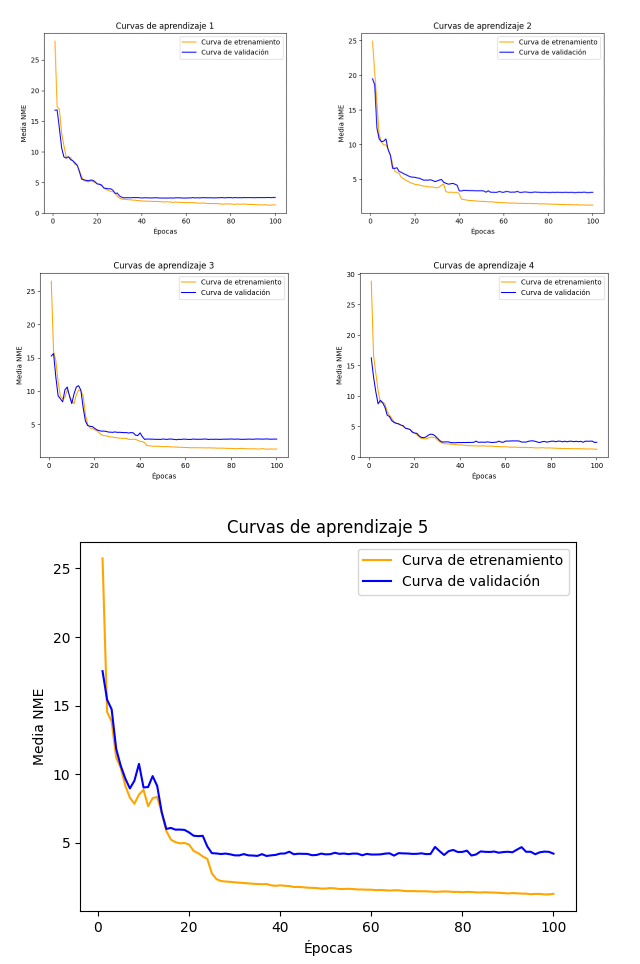
\includegraphics[width=0.9\textwidth]{img/curvas_decoder.png}
            \caption{Curvas de aprendizaje en cada partición del modelo de finetuning del encoder.}
            \label{fig:curvas_decoder}
        \end{figure}

        \medskip

        \noindent Tras los resultados obtenidos se ha optado por abandonar también esta línea de investigación pues se obtienen resultados muy similares al modelo base y se debe entrenar por mucho más tiempo ($100$ épocas frente a $40$ del modelo base). Los resultados del modelo sobre algunas imágenes pueden verse en \autoref{fig:Ejemplo_decoder}

        \begin{figure}[H]
            \centering
            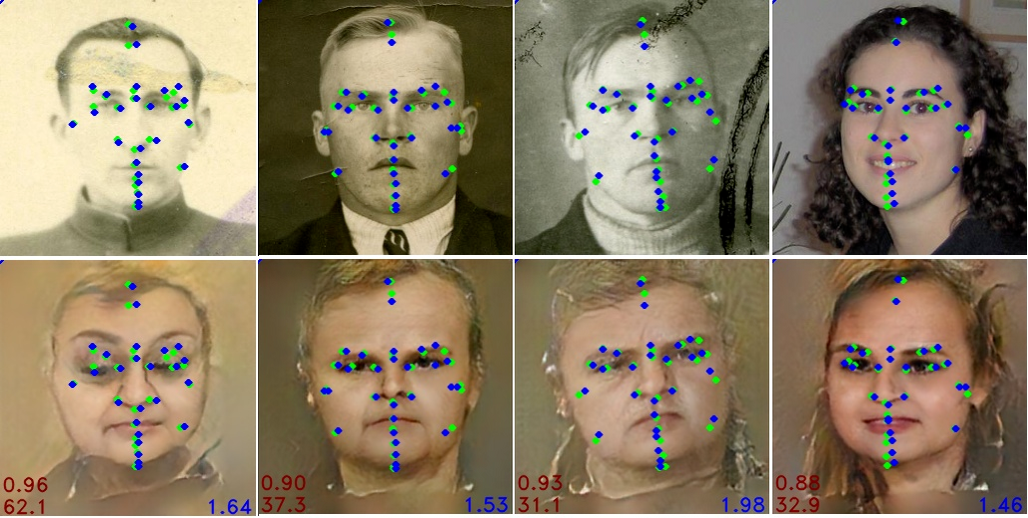
\includegraphics[width=0.9\textwidth]{img/image_decoder.png}
            \caption{Imágenes pertenecientes a distintos conjuntos de validación para el \textbf{modelo de ajuste fino del decoder}.}
            \label{fig:Ejemplo_decoder}
        \end{figure}

    \subsection{Modelo con Data Augmentation}
        \noindent Vamos a optar a continuación por un nuevo enfoque. En lugar de mejorar el error de reconstrucción vamos a centrarnos en mejorar el marcado de landmarks en las imágenes reconstruidas que genera el modelo preentrenado. Como pudimos ver en el modelo base, se consiguieron buenos resultados del \textit{NME} pese a haber entrenado sin realizar técnicas de \textit{data augmentation}. Es por ello que en este segundo experimento vamos a realizar los siguientes cambios en el entrenamiento: 
        
        \begin{itemize}
            \item En primer lugar se realizará un entrenamiento del modelo similar al del modelo base durante $40$ épocas.
            \item Tras esto, se entrenará el modelo con el dataset al cual se le aplicarán técnicas de data augmentation, para aumentar el número de datos de entrenamiento e incrementar aún más la variabilidad de los mismos, de manera que cada imagen del dataset sufrirá de manera aleatoria una traslación ($\pm 4\%$), un reescalado ($\pm 5\%$), una rotación ($\pm 30$ grados) y oclusiones parciales. El entrenamiento en este nuevo dataset será durante $40$ épocas tras acabar las de la etapa anterior.
            \item En total serán \textbf{$80$ épocas} de entrenamiento sumando las dos etapas anteriores.
        \end{itemize}

        \medskip

        \noindent De nuevo, el resto de parámetros continuarán con los valores por defecto de la etapa anterior, pues los resultados obtenidos han sido buenos hasta el momento y nada sugiere tener que cambiarlos.

        \begin{table}[!ht]
            \centering
            \caption{Tabla comparativa entre todos los modelos probados.}
            \begin{tabular}{|l|l|l|l|l|l|}
            \hline
                \textbf{} & \cellcolor{gray!25}\textbf{Landmark} & \cellcolor{gray!25}\textbf{M.Base} & \cellcolor{gray!25}\textbf{M.E} & \cellcolor{gray!25}\textbf{M.Decoder} & \cellcolor{gray!25}\textbf{Data augmentation} \\ \hline
                \textbf{0} & Menton & 3.944 & 3.997 & 3.991 & \cellcolor{green!25}3.006 \\ \hline
                \textbf{1} & Gnathion & 2.637 & 2.606 & 2.634 & \cellcolor{green!25}1.497 \\ \hline
                \textbf{2} & Pogonion & 2.549 & 2.546 & 2.585 & \cellcolor{green!25}1.359 \\ \hline
                \textbf{3} & Prosthion & 0.932 & 1.048 & 0.97 & \cellcolor{green!25}0.815 \\ \hline
                \textbf{4} & Labiale Superius & 2.099 & 2.04 & 2.059 & \cellcolor{green!25}1.531 \\ \hline
                \textbf{5} & Subnasale & 2.059 & 1.992 & 2.089 & \cellcolor{green!25}1.272 \\ \hline
                \textbf{6} & Nasion & 2.254 & 2.099 & 2.275 & \cellcolor{green!25}1.241 \\ \hline
                \textbf{7} & Glabella & 2.547 & 2.736 & 2.912 & \cellcolor{green!25}1.545 \\ \hline
                \textbf{8} & Vertex & 6.244 & 5.89 & 6.137 & \cellcolor{green!50}\textbf{3.99} \\ \hline
                \textbf{9} & Left Gonion & 7.684 & 5.789 & 5.665 & \cellcolor{green!50}\textbf{1.846} \\ \hline
                \textbf{10} & Right Gonion & 11.283 & 5.301 & 5.468 & \cellcolor{green!50}\textbf{1.673} \\ \hline
                \textbf{11} & Left Zygion & 5.098 & 5.288 & 5.29 & \cellcolor{green!50} \textbf{3.322} \\ \hline
                \textbf{12} & Right Zygion & 6.309 & 6.291 & 6.14 & \cellcolor{green!50} \textbf{4.441} \\ \hline
                \textbf{13} & Left Alare & 1.939 & 1.959 & 2.051 & \cellcolor{green!25}1.585 \\ \hline
                \textbf{14} & Right Alare & 2.282 & 2.232 & 2.295 & \cellcolor{green!25}1.362 \\ \hline
                \textbf{15} & Left Endocanthion & 1.668 & 1.71 & 1.827 & \cellcolor{green!25}1.227 \\ \hline
                \textbf{16} & Right Endocanthion & 1.671 & 1.647 & 1.61 & \cellcolor{green!25}1.129 \\ \hline
                \textbf{17} & Left Exocanthion & 1.706 & 1.733 & 1.809 & \cellcolor{green!25}1.186 \\ \hline
                \textbf{18} & Right Exocanthion & 1.670 & 1.746 & 1.734 & \cellcolor{green!25}1.12 \\ \hline
                \textbf{19} & Left Tragion & 4.824 & 3.633 & 4.163 & \cellcolor{green!25}2.066 \\ \hline
                \textbf{20} & Right Tragion & 5.376 & 5.252 & 4.791 & \cellcolor{green!25}2.234 \\ \hline
                \textbf{21} & Labiale inferius & 1.705 & 1.688 & 1.627 & \cellcolor{green!25}1.032 \\ \hline
                \textbf{22} & Trichion & 4.478 & 4.762 & 5.196 & \cellcolor{green!25} 3.37 \\ \hline
                \textbf{23} & Supramentale & 1.913 & 1.991 & 1.839 & \cellcolor{green!25}1.109 \\ \hline
                \textbf{24} & Left Frontotemporale & 2.319 & 2.452 & 2.474 & \cellcolor{green!25}1.386 \\ \hline
                \textbf{25} & Right Frontotemporale & 2.721 & 3.282 & 3.009 & \cellcolor{green!25}1.826 \\ \hline
                \textbf{26} & Left Frontozygomaticus & 1.513 & 1.499 & 1.525 & \cellcolor{green!25}1.036 \\ \hline
                \textbf{27} & Right Frontozygomaticus & 2.313 & 2.516 & 2.395 & \cellcolor{green!25}1.057 \\ \hline
                \textbf{28} & Left Midsurpaorbital & 1.205 & 1.178 & 1.191 & \cellcolor{green!25}0.854 \\ \hline
                \textbf{29} & Right Midsupraorbital & 1.43 & 1.348 & 1.48 & \cellcolor{green!25}0.945 \\ \hline
            \end{tabular}
            \label{table:Daugmentation_landmarksresume}
        \end{table}
        \medskip

        \noindent Como podemos ver en la \autoref{table:Daugmentation_landmarksresume}, los errores se han reducido en todos los landmarks. Además, la red ha conseguido aprender a marcar con un alto grado de precisión los puntos que se ven en el perfil de la cara también, siendo esta alternativa menos costosa que la de los dos modelos anteriores tanto en número de épocas como en parámetros que se actualizan de la red (en este nuevo modelo sólo se actualizan los pesos de las ITLs). El punto mejor marcado sería el \textit{prosthion} de nuevo, y el peor marcado el \textit{right zygion}. Sin embargo, la diferencia en términos de error entre ambos es mucho menor que en el caso del modelo base. 

        \medskip

        \noindent En lo que se refiere al error por imagen, como podemos ver en el \autoref{ap:apendiceD}, el error desciende mucho en comparación con los modelos anteriores pese a que el de reconstrucción continua elevado.

        \medskip

        \noindent Finalmente las curvas de aprendizaje obtenidas se pueden observar en \autoref{fig:curvas_daugmentation}. Como vemos presentan una gran capacidad de generalización, pues el error de entrenamiento y validación decrecen de forma continua y muy próxima. Algunas imágenes de ejemplo podemos verlas en la \autoref{fig:Ejemplo_daug}.

        \begin{figure}[H]
            \centering
            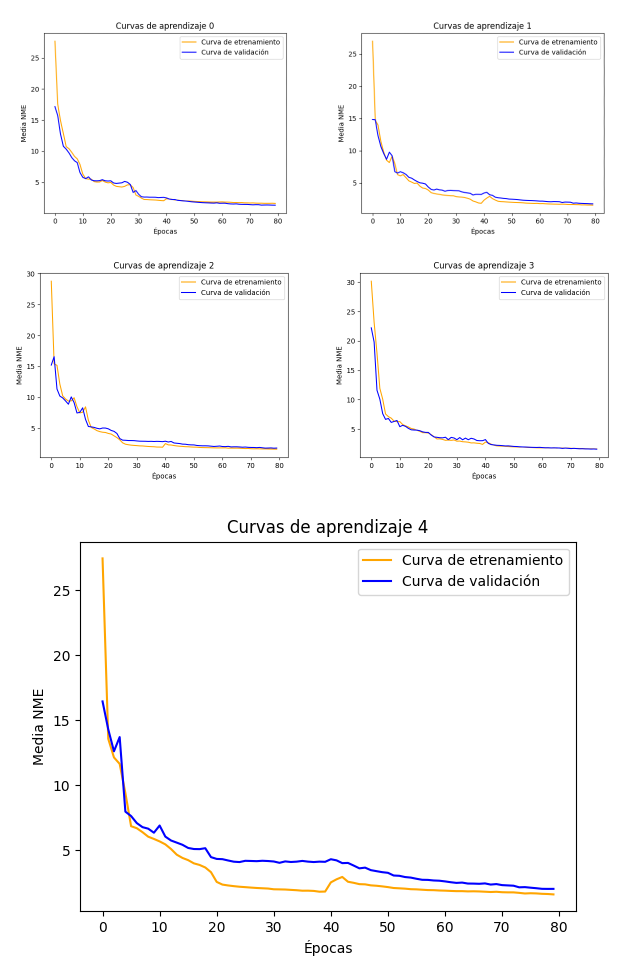
\includegraphics[width=0.9\textwidth]{img/curvas_daugmentation.png}
            \caption{Curvas de aprendizaje en cada partición del modelo de data augmentation.}
            \label{fig:curvas_daugmentation}
        \end{figure}

        \begin{figure}[H]
            \centering
            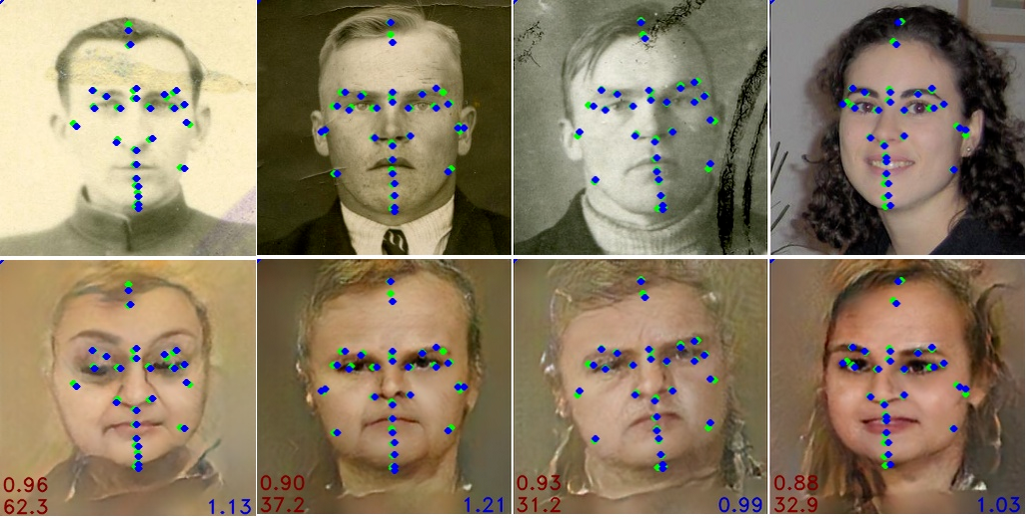
\includegraphics[width=0.9\textwidth]{img/image_daug.png}
            \caption{Imágenes pertenecientes a distintos conjuntos de validación para el \textbf{modelo data augmentation}.}
            \label{fig:Ejemplo_daug}
        \end{figure}

    \subsection{Elección de modelo y obtención de resultados}

        \noindent Una vez analizados los distintos modelos que se proponen para resolver el problema, vemos que la alternativa más prometedora resulta ser la última, la de aplicar técnicas de \textit{data augmentation} al dataset. Es por ello que ahora tomaremos el conjunto de entrenamiento en su totalidad (sin realizar particiones como hicimos para \textit{cross validation}) y vamos a usarlo para entrenar el modelo durante las mismas épocas que en la sección anterior y con los mismos parámetros y transformaciones. Posteriormente usaremos el conjunto de test de $33$ imágenes que separamos al principio de esta sección, y que hasta ahora no hemos visto para evitar \textit{data snooping}, para validar el modelo.

        \begin{table}[!ht]
            \centering
            \caption{Tabla comparativa entre los resultados del modelo de data augmentation en el conjunto de validación y test}
            \begin{tabular}{|l|l|l|}
            \hline
                \cellcolor{gray!25}\textbf{Landmark} & \cellcolor{gray!25}\textbf{NME Test} & \cellcolor{gray!25}\textbf{NME Validación} \\ \hline
                \textbf{Menton} & \cellcolor{green!25}0.946 & 3.006 \\ \hline
                \textbf{Gnathion} & 3.323 & \cellcolor{green!25}1.497 \\ \hline
                \textbf{Pogonion} & 3.149 & \cellcolor{green!25}1.359 \\ \hline
                \textbf{Prosthion} & 0.89 & \cellcolor{green!25}0.815 \\ \hline
                \textbf{Labiale Superius} & \cellcolor{green!25}1.134 & 1.531 \\ \hline
                \textbf{Subnasale} & 2.982 & \cellcolor{green!25}1.272 \\ \hline
                \textbf{Nasion} & 3.1 & \cellcolor{green!25}1.241 \\ \hline
                \textbf{Glabella} & 3.089 & \cellcolor{green!25}1.545 \\ \hline
                \textbf{Vertex} & 6.568 & \cellcolor{green!25}3.99 \\ \hline
                \textbf{Left Gonion} & 4.334 & \cellcolor{green!25}1.846 \\ \hline
                \textbf{Right Gonion} & \cellcolor{green!25}1.297 & 1.673 \\ \hline
                \textbf{Left Zygion} & 4.813 & \cellcolor{green!25}3.322 \\ \hline
                \textbf{Right Zygion} & 4.465 & \cellcolor{green!25}4.441 \\ \hline
                \textbf{Left Alare} & 3.531 & \cellcolor{green!25}1.585 \\ \hline
                \textbf{Right Alare} & 3.641 & \cellcolor{green!25}1.362 \\ \hline
                \textbf{Left Endocanthion} & 3.917 & \cellcolor{green!25}1.227 \\ \hline
                \textbf{Right Endocanthion} & 4.685 & \cellcolor{green!25}1.129 \\ \hline
                \textbf{Left Exocanthion} & 3.936 & \cellcolor{green!25}1.186 \\ \hline
                \textbf{Right Exocanthion} & 4.526 & \cellcolor{green!25}1.12 \\ \hline
                \textbf{Left Tragion} & 2.365 & \cellcolor{green!25}2.066 \\ \hline
                \textbf{Right Tragion} & \cellcolor{green!25}1.678 & 2.234 \\ \hline
                \textbf{Labiale inferius} & 1.083 & \cellcolor{green!25}1.032 \\ \hline
                \textbf{Trichion} & \cellcolor{green!25}1.731 & 3.37 \\ \hline
                \textbf{Supramentale} & \cellcolor{green!25}1.064 & 1.109 \\ \hline
                \textbf{Left Frontotemporale} & \cellcolor{green!25}1.208 & 1.386 \\ \hline
                \textbf{Right Frontotemporale} & \cellcolor{green!25}1.282 & 1.826 \\ \hline
                \textbf{Left Frontozygomaticus} & \cellcolor{green!25}1.024 & 1.036 \\ \hline
                \textbf{Right Frontozygomaticus} & \cellcolor{green!25}0.943 & 1.057 \\ \hline
                \textbf{Left Midsurpaorbital} & \cellcolor{green!25}0.846 & 0.854 \\ \hline
                \textbf{Right Midsupraorbital} & 2.027 & \cellcolor{green!25}0.945 \\ \hline
            \end{tabular}
            \label{table:FinalModel_landmarks}
        \end{table}
        
        \medskip

        \noindent En primer lugar, como se puede apreciar en la \autoref{table:FinalModel_landmarks} obtenemos: 

        \begin{itemize}
            \item En general los landmarks empeoran ligeramente su error NME. Esto es normal pues en la etapa anterior todas las decisiones para mejorar los modelos se tomaron en función de los resultados de validación. Sin embargo estos datos nuevos en los que se está probando el modelos no han sido estudiados previamente, por lo que es normal que baje el rendimiento. No obstante, los resultados siguen siendo buenos, y no se empeoran excesivamente en la mayoría de casos. 
            \item En total empeoran su error $19$ de los $30$ landmarks marcados. En algunos casos el error se duplica, como puede ser el \textit{Gnation} y en otros empeora levemente, como ocurre con el \textit{Left Zygion}. 
            \item En total mejoran su error $11$ de los $30$ landmarks, destacando la importante mejora en la identificación del \textit{Menton}, y algunas más leves como las del \textit{Right/Left Frontotemporale}.
        \end{itemize}

        \medskip

        \noindent Por otro lado, las curvas de aprendizaje durante el entrenamiento del modelo se pueden observar en la \autoref{fig:curvas_FinalModel}. En ellas podemos observar una mayor distancia entre la curva de entrenamiento y validación, fruto de nuevo de no haber usado el conjunto de test para tomar decisiones, como si que hicimos con los datos de validación en \textit{cross-validation}. Podemos ver el rendimiento del modelo en algunas imágenes en \autoref{fig:Ejemplo_finalmodel}.

        \begin{figure}[H]
            \centering
            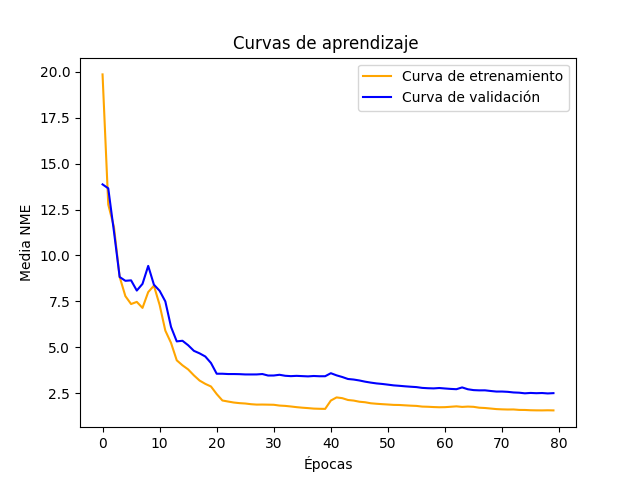
\includegraphics[width=0.9\textwidth]{img/curvas_FinalModel.png}
            \caption{Curvas de aprendizaje durante el entrenamiento del modelo de data augmentation validado en el conjunto de test.}
            \label{fig:curvas_FinalModel}
        \end{figure}

        \begin{figure}[H]
            \centering
            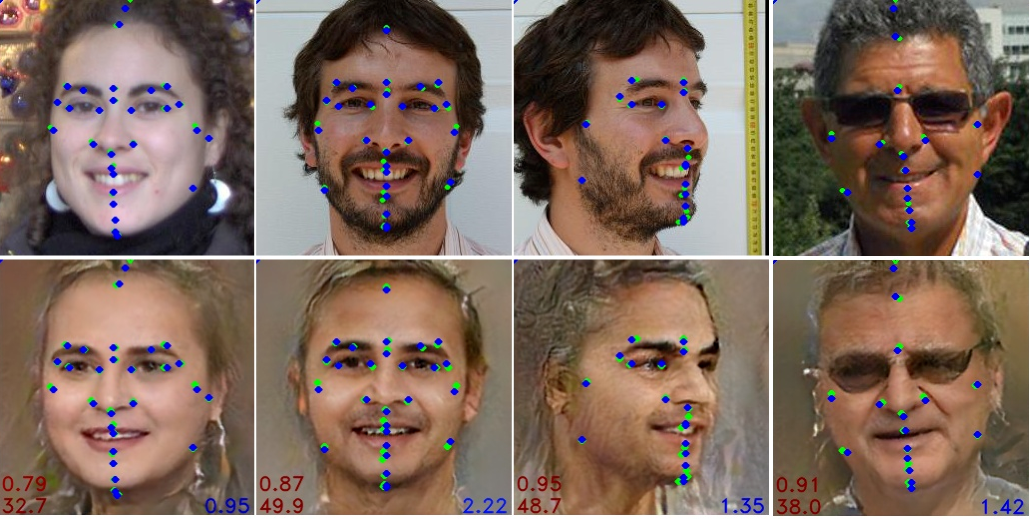
\includegraphics[width=0.9\textwidth]{img/image_finalmodel.png}
            \caption{Rendimiento del modelo final elegido con data augmentation en imágenes del conjunto de test.}
            \label{fig:Ejemplo_finalmodel}
        \end{figure}

        \medskip

        \noindent Como podemos ver, en general el modelo se comporta bien en la tarea del reconocimiento de landmarks, es capaz de predecirlos con una tasa de error NME muy pequeña, por lo que podemos concluir que el modelo resuleve la tarea que nos habíamos propuesto con éxito. No obstante, el éxito real del modelo debe supervisarlo un experto forense, pues no sabemos si los errores cometidos en la identificación de landmarks son errores asumibles o si se requiere un mayor grado de precisión.

    \section{Comparativa entre 3FabRec y HyperFace-ResNet101}
        \noindent Vamos a comparar ahora el modelo final obtenido a partir de \textbf{3FabRec} con otro que fue diseñado para el mismo propósito basado en \textbf{HyperFace-Resnet101}, otra red especializada en el marcado de landmarks, realizado por Guillermo Gómez.

        \subsection{Preprocesamiento y base de datos empleada}
            \noindent En lo que respecta al preprocesamiento de los datos, nuestro modelo basado en \textit{3FabRec} únicamente emplea como etapa de preprocesamiento la identificación de bounding boxes en el conjunto de datos inicial de cara a poder entrenar la red. Por otro lado, este estudio se limita a usar las $167$ imágenes proporcionadas.

            \medskip

            \noindent En cambio, el modelo basado en \textit{HF-ResNet} además de emplear también un detector de caras para los bounding boxes, contaba con un dataset auxiliar de modelos $3D$ de personas sobre las que estaban marcados $27$ de los $30$ landmarks que se predicen. Lo cual sirvió para aumentar el conjunto de datos de entrenamiento realizando proyecciones $2D$ a partir de estos modelos.

        \subsection{Métricas empleadas}
            \noindent La métrica empleada en el trabajo dónde se presenta el modelo es el \textbf{RMSE}. Se trata de la raíz del error cuadrático medio y su expresión es la siguiente: 

            \begin{equation}
                RMSE(y,\widehat{y})= \sqrt{\frac{1}{N} \sum_{i=1}^{N} (y_i-\widehat{y}_i)^2}
            \end{equation}

            \noindent donde $y_i$ representa las coordenadas del landmark real y $\widehat{y_i}$ el predicho homólogo número $i$ del total de $N$ landmarks marcados.

            \medskip

            \noindent Para poder realizar una comparación entre ambos métodos, se extrae esta métrica del rendimiento del modelo final en el conjunto de test. 

        \subsection{Comparación de resultados}
            \noindent En primer lugar comparamos ambos modelos calculando la mediana del \textit{RMSE} producido en cada landmark, así como los percentiles $25$, $50$ y $75$. Podemos ver estos resultados en la \autoref{table:comparativa-global}.

            \begin{table}[!ht]
                \centering
                \caption{Tabla comparativa a nivel global entre los dos modelos. Como podemos observar, el modelo basado en \textbf{HyperFace-Resnet101} obtiene mejores resultados en global en todos los campos.}
                \begin{tabular}{|l|l|l|l|l|}
                \hline
                    \cellcolor{gray!25}\textbf{Modelo} & \cellcolor{gray!25}\textbf{RMSE} & \cellcolor{gray!25}\textbf{P25} & \cellcolor{gray!25}\textbf{P50} & \cellcolor{gray!25}\textbf{P75} \\ \hline
                    \textbf{Modelo HyperFace-Resnet101} & \cellcolor{green!25}3.4106 & \cellcolor{green!25}1.802 & \cellcolor{green!25}2.7569 & \cellcolor{green!25}4.2849 \\ \hline
                    \textbf{Modelo 3FabRec} & 5.3862 & 3.0991 & 5.3862 & 5.9819 \\ \hline
                \end{tabular}
                \label{table:comparativa-global}
            \end{table}
            
            \medskip

            \noindent A nivel general, parece que el modelo basado en \textit{HyperFace-ResNet101} es mejor que el presentado en este trabajo, no obstante vamos a realizar una comparativa a nivel de landmark entre los dos modelos. Podemos ver esta comparativa en la \autoref{table:comparativa-Landmarks}.
            \begin{table}[!ht]
                \centering
                \caption{Tabla comparativa a nivel de landmarks entre el modelo final basado en 3FabRec y el de HyperFace-REsNet101.}
                \begin{tabular}{|l|l|l|}
                \hline
                    \cellcolor{gray!25}\textbf{Landmark} & \cellcolor{gray!25}\textbf{RMSE 3FabRec} & \cellcolor{gray!25}\textbf{RMSE HyperFace-Resnet101} \\ \hline
                    \textbf{Menton} & 6.43 & \cellcolor{green!25} 4.97 \\ \hline
                    \textbf{Gnathion} & 5.5 & \cellcolor{green!25}3.84 \\ \hline
                    \textbf{Pogonion} & 5.5 & \cellcolor{green!25}3.99 \\ \hline
                    \textbf{Prosthion} & \cellcolor{green!25}1.73 & 3.23 \\ \hline
                    \textbf{Labiale Superius} & 3.35 & \cellcolor{green!25}2.35 \\ \hline
                    \textbf{Subnasale} & 4.9 & \cellcolor{green!25}3.33 \\ \hline
                    \textbf{Nasion} & 4.91 & \cellcolor{green!25}3.12 \\ \hline
                    \textbf{Glabella} & 5.36 & \cellcolor{green!25}3.89 \\ \hline
                    \textbf{Vertex} & 10.95 & \cellcolor{green!25}8.83 \\ \hline
                    \textbf{Left Gonion} & 9.7 & \cellcolor{green!25}7.12 \\ \hline
                    \textbf{Right Gonion} & 7.23 & \cellcolor{green!25}6.11 \\ \hline
                    \textbf{Left Zygion} & 11.49 & \cellcolor{green!25}5.78 \\ \hline
                    \textbf{Right Zygion} & 13.47 & \cellcolor{green!25}6.94 \\ \hline
                    \textbf{Left Alare} & 5.6 & \cellcolor{green!25}3.50 \\ \hline
                    \textbf{Right Alare} & 5.68 & \cellcolor{green!25}2.84 \\ \hline
                    \textbf{Left Endocanthion} & 5.11 & \cellcolor{green!25}2.40 \\ \hline
                    \textbf{Right Endocanthion} & 6.0 & \cellcolor{green!25}2.32 \\ \hline
                    \textbf{Left Exocanthion} & 6.11 & \cellcolor{green!25}3.73 \\ \hline
                    \textbf{Right Exocanthion} & 5.92 & \cellcolor{green!25}3.62 \\ \hline
                    \textbf{Left Tragion} & \cellcolor{green!25}5.34 & 7.01 \\ \hline
                    \textbf{Right Tragion} & \cellcolor{green!25}5.81 & 6.41 \\ \hline
                    \textbf{Labiale inferius} & \cellcolor{green!25}2.43 & 3.11 \\ \hline
                    \textbf{Trichion} & \cellcolor{green!25}5.41 & 7.02 \\ \hline
                    \textbf{Supramentale} & \cellcolor{green!25}2.29 & 3.43 \\ \hline
                    \textbf{Left Frontotemporale} & \cellcolor{green!25}3.16 & 3.78 \\ \hline
                    \textbf{Right Frontotemporale} & \cellcolor{green!25}3.08 & 3.27 \\ \hline
                    \textbf{Left Frontozygomaticus} & \cellcolor{green!25}2.25 & 2.75 \\ \hline
                    \textbf{Right Frontozygomaticus} & \cellcolor{green!25}2.2 & 2.80 \\ \hline
                    \textbf{Left Midsurpaorbital} & \cellcolor{green!25}1.91 & 2.57 \\ \hline
                    \textbf{Right Midsupraorbital} & 3.05 & \cellcolor{green!25}2.24 \\ \hline
                \end{tabular}
                \label{table:comparativa-Landmarks}
            \end{table}

            \medskip
            
            \begin{itemize}
                \item En total $11$ landmarks se marcan con mayor precisión con el modelo basado en \textbf{3FabRec}.
                \item En total $19$ landmarks se marcan mejor en con el modelo basado en \textbf{HyperFace-ResNet101}.
            \end{itemize}

            \noindent Como podemos observar, en su mayoría los landmarks que el modelo basado en \textit{HyperFace-ResNet101} son más precisos que los marcados por nuestro modelo en una media de $2$ píxeles de diferencia.
           
\endinput
%------------------------------------------------------------------------------------
% FIN DEL CAPÍTULO. 
%------------------------------------------------------------------------------------



